\documentclass[]{elsarticle} %review=doublespace preprint=single 5p=2 column
%%% Begin My package additions %%%%%%%%%%%%%%%%%%%
\usepackage[hyphens]{url}

  \journal{Journal of Applied Ecology} % Sets Journal name


\usepackage{lineno} % add
\providecommand{\tightlist}{%
  \setlength{\itemsep}{0pt}\setlength{\parskip}{0pt}}

\usepackage{graphicx}
%%%%%%%%%%%%%%%% end my additions to header

\usepackage[T1]{fontenc}
\usepackage{lmodern}
\usepackage{amssymb,amsmath}
\usepackage{ifxetex,ifluatex}
\usepackage{fixltx2e} % provides \textsubscript
% use upquote if available, for straight quotes in verbatim environments
\IfFileExists{upquote.sty}{\usepackage{upquote}}{}
\ifnum 0\ifxetex 1\fi\ifluatex 1\fi=0 % if pdftex
  \usepackage[utf8]{inputenc}
\else % if luatex or xelatex
  \usepackage{fontspec}
  \ifxetex
    \usepackage{xltxtra,xunicode}
  \fi
  \defaultfontfeatures{Mapping=tex-text,Scale=MatchLowercase}
  \newcommand{\euro}{€}
\fi
% use microtype if available
\IfFileExists{microtype.sty}{\usepackage{microtype}}{}
\usepackage[margin=1.1in]{geometry}
\bibliographystyle{elsarticle-harv}
\usepackage{longtable,booktabs,array}
\usepackage{calc} % for calculating minipage widths
% Correct order of tables after \paragraph or \subparagraph
\usepackage{etoolbox}
\makeatletter
\patchcmd\longtable{\par}{\if@noskipsec\mbox{}\fi\par}{}{}
\makeatother
% Allow footnotes in longtable head/foot
\IfFileExists{footnotehyper.sty}{\usepackage{footnotehyper}}{\usepackage{footnote}}
\makesavenoteenv{longtable}
\ifxetex
  \usepackage[setpagesize=false, % page size defined by xetex
              unicode=false, % unicode breaks when used with xetex
              xetex]{hyperref}
\else
  \usepackage[unicode=true]{hyperref}
\fi
\hypersetup{breaklinks=true,
            bookmarks=true,
            pdfauthor={},
            pdftitle={Quantifying mesopredator release: lethal control of an invasive apex predator alters feral cat density and detectability},
            colorlinks=false,
            urlcolor=blue,
            linkcolor=magenta,
            pdfborder={0 0 0}}
\urlstyle{same}  % don't use monospace font for urls

\setcounter{secnumdepth}{5}
% Pandoc toggle for numbering sections (defaults to be off)

% Pandoc citation processing

% Pandoc header
\usepackage{setspace}\doublespacing
\usepackage{float}
\floatplacement{figure}{H}
\newcommand{\beginsupplement}{\setcounter{table}{0}  \renewcommand{\thetable}{S\arabic{table}} \setcounter{figure}{0} \renewcommand{\thefigure}{S\arabic{figure}} \setcounter{section}{0} \renewcommand{\thesection}{S\arabic{section}}}
\usepackage{lineno}
\usepackage{booktabs}
\usepackage{longtable}
\usepackage{array}
\usepackage{multirow}
\usepackage{wrapfig}
\usepackage{float}
\usepackage{colortbl}
\usepackage{pdflscape}
\usepackage{tabu}
\usepackage{threeparttable}
\usepackage{threeparttablex}
\usepackage[normalem]{ulem}
\usepackage{makecell}
\usepackage{xcolor}



\begin{document}
\begin{frontmatter}

  \title{Quantifying mesopredator release: lethal control of an invasive apex predator alters feral cat density and detectability}
    \author[UOM]{Matthew W. Rees\corref{1}}
   \ead{matt.wayne.rees@gmail.com} 
    \author[CEC]{Jack H. Pascoe}
  
    \author[CEC]{Mark Le Pla}
  
    \author[ARI]{Alan Robley}
  
    \author[CEC]{Emma K. Birnbaum}
  
    \author[UOM]{Brendan A. Wintle}
  
    \author[UOM]{Bronwyn A. Hradsky}
  
      \address[UOM]{Quantitative \& Applied Ecology Group, School of Ecosystem and Forest Science, The University of Melbourne, Parkville, VIC, Australia}
    \address[CEC]{Conservation Ecology Centre, Otway Lighthouse Rd, Cape Otway, VIC, Australia}
    \address[ARI]{Department of Environment, Land, Water and Planning, Arthur Rylah Institute for Environmental Research, Heidelberg, Australia}
      \cortext[1]{Corresponding Author}
  
  \begin{abstract}
  
  \end{abstract}
   \begin{keyword} feral cat; invasive predator; mesopredator release; population density; red fox; spatial capture-recapture; species interactions; 1080 poison\end{keyword}
 \end{frontmatter}

\parskip=12pt

\emph{Article type}: Research Article

\emph{Running title}: Invasive mesopredator release

\emph{Word count (abstract, body)}: 321, 5620

\emph{References}: 71

\emph{Figures}: 6

\emph{Tables}: 0

\emph{Authorship}: M.W.R, B.A.H, J.H.P, B.A.W and A.R conceived the ideas and designed the methodology; M.W.R, J.H.P, M.LP, E.K.B and B.A.H collected the data; M.W.R analysed the data with input from B.A.H and B.A.W, and led the writing of the manuscript. All authors contributed critically to the drafts and gave final approval for publication.

\emph{Data accessibility}: Data and code will be deposited on the Dryad Digital Repository after acceptance and can be viewed here: \url{https://github.com/matt-w-rees/invasive-mesopredator-release}.

\newpage

\linenumbers

\hypertarget{abstract}{%
\section*{ABSTRACT}\label{abstract}}
\addcontentsline{toc}{section}{ABSTRACT}

\begin{enumerate}
\def\labelenumi{\arabic{enumi}.}
\item
  The mesopredator release hypothesis predicts that subordinate predator density will increase as apex predators decline. Persistent debate around mesopredator release in part reflects the lack of robust, replicated experiments to test this theory, and the use of population indices which confound changes in mesopredator density and detectability. This uncertainty has immediate impacts for conservationists who are faced with managing sympatric invasive predators.
\item
  We used replicating experimental designs and spatially explicit detection modelling to examine whether mesopredator release of the feral cat \emph{Felis catus} occurs in response to targeted control of the introduced red fox \emph{Vulpes vulpes}. We surveyed three Control-Impact paired landscapes in a region with long-term fox control (1080 poison-baiting), and conducted a Before-After-Control-Impact Paired Series experiment in another region. We identified 160 individual feral cats from 68,504 camera-trap nights to estimate feral cat density with spatial mark-resight models.
\item
  At a landscape scale (mean size: 169 km\textsuperscript{2}), lethal fox control was associated with a range of responses from a negligible to 3.7-fold increase in feral cat density. Consistent with the mesopredator release hypothesis, the degree of increase corresponded with variation in the duration and intensity of fox suppression. At a fine spatial scale (200 m), feral cat density had a consistent negative association with fox activity across both regions.
\item
  Feral cat detectability also varied across the (artificially manipulated) fox activity gradient. In one region, nonlinear models indicated that feral cats exhibited avoidance behaviours when foxes were rare, giving way to density suppression at high fox activity.
\item
  \emph{Synthesis and applications.} Our study provides replicated, experimental evidence that that apex predator suppression is associated with an increase in the density of a mesopredator. Mesopredator release can manifest as changes in both behaviour and density, distorting inference if these processes are not distinguished. Our results help explain why fox control does not consistently improve native prey persistence, suggesting integrated pest management may be necessary to improve conservation outcomes.
\end{enumerate}

\newpage

\hypertarget{introduction}{%
\section{INTRODUCTION}\label{introduction}}

Understanding species interactions is critical for effective invasive species management (Zavaleta, Hobbs, \& Mooney 2001). When several invasive species co-occur, management actions that suppress the dominant invasive species may inadvertently benefit subordinate invasive species (Jackson 2015; Kuebbing \& Nuñez 2015). For example, the removal of a dominant invasive predator may increase the abundance of a subordinate invasive species directly by reducing top-down pressure, or indirectly by increasing the availability of shared resources; these are often referred to as mesopredator or competitor release, respectively (Crooks \& Soulé 1999; Ruscoe \emph{et al.} 2011; Doherty \& Ritchie 2017). The release of subordinate invasive species, particularly predators, can have serious negative implications for native taxa and ecosystem function (Courchamp, Langlais, \& Sugihara 1999; Ballari, Kuebbing, \& Nuñez 2016). However, integrated invasive predator management is often far more costly and less feasible than single species control, and so it is important to identify when the extra cost is justified (Bode, Baker, \& Plein 2015).

Most knowledge of mesopredator release stems from unreplicated `natural experiments' (e.g.~range contractions - Crooks \& Soulé 1999) or ad-hoc management interventions (e.g.~invasive species eradications - Rayner \emph{et al.} 2007). Does mesopredator release still occur when apex predators are suppressed but not completely removed? The occurrence, nature (positive or negative, direct or indirect) and strength of predator interactions can vary among species assemblages, predation risk, environmental productivity, management regimes and other landscape contexts (Hastings 2001; Finke \& Denno 2004; Elmhagen \& Rushton 2007; Newsome \emph{et al.} 2017; Alston \emph{et al.} 2019). Replicating management programs in an experimental framework is logistically challenging, but important for understanding these complexities, discriminating between plausible hypotheses and producing generalisable results to inform effective pest management (Glen \& Dickman 2005; Hayward \emph{et al.} 2015; Christie \emph{et al.} 2019; Smith \emph{et al.} 2020).

Another source of uncertainty around the mesopredator release hypothesis stems from the inability of traditional survey and modelling approaches to distinguish behavioural from numerical population processes (Hayward \emph{et al.} 2015; Stephens \emph{et al.} 2015). Suppression of an apex predator may simultaneously change the behaviour and the density of a mesopredator, both of which influence detection rates (Broadley \emph{et al.} 2019; Rogan \emph{et al.} 2019). This makes it difficult to interpret observed changes in naive indices of mesopredator activity or occupancy in relation to changes in apex predator populations, even if the study has an experimental design. Unbiased estimates of invasive predator density are also important for setting meaningful control targets and inferring impacts on native prey (Moseby \emph{et al.} 2019). Spatial capture-recapture methods offer a solution by separating behavioural and observational processes from population density, which is estimated within a defined spatial resolution (Borchers \& Efford 2008).

Predation by two invasive species, the red fox \emph{Vulpes vulpes} (hereafter `fox') and feral cat \emph{Felis catus} (hereafter `cat'), has played a major role in Australia's high rates of mammalian extinction (Woinarski, Burbidge, \& Harrison 2015). Integrated pest management programs are rare; instead, foxes are far more commonly controlled than cats, as they are more susceptible to poison-baiting, have greater direct economic impacts and fewer legal impediments to control (Reddiex \emph{et al.} 2007; McLeod \& Saunders 2014). Nonetheless, cats are one of the most widespread and damaging vertebrate predator species (Medina \emph{et al.} 2011; Doherty \& Ritchie 2017; Legge \emph{et al.} 2020). As foxes are larger-bodied (\textasciitilde2 kg difference) and have high dietary overlap with cats (Stobo-Wilson \emph{et al.} 2021a; b), the mesopredator release hypothesis (Soulé \emph{et al.} 1988) predicts that the impacts of cats on shared prey species will increase as fox populations are suppressed. This is alarming because feral cats are extremely difficult to manage in open populations (Fisher \emph{et al.} 2015; Lazenby, Mooney, \& Dickman 2015).

Evidence that foxes suppress cats is inconclusive (Hunter \emph{et al.} 2018). In parts of Australia where the native apex mammalian predator (the dingo \emph{Canis familiaris}) is functionally extinct and introduced foxes are the largest terrestrial mammalian predator, four studies have observed an increase in cat detections following fox control (Risbey \emph{et al.} 2000; Marlow \emph{et al.} 2015; Stobo-Wilson \emph{et al.} 2020). However, two other studies in similar systems did not see any change (Towerton \emph{et al.} 2011; Molsher \emph{et al.} 2017). A further study with spatial replication detected an increase at one site but not another (Davey \emph{et al.} 2006), and another observed a decrease in cat activity (Claridge \emph{et al.} 2010). No prior studies have directly estimated cat density in response to fox control.

We experimentally investigated the role of introduced foxes in top-down suppression of cat density in two regions of south-eastern Australia. Our experiments had a replicated Control-Impact design in the region with long-term fox control, and a Before-After Control-Impact Paired Series (BACIPS) design in the region with newly implemented fox control. Foxes and cats are the only functional terrestrial mammalian predators in these regions, and each region included at least one area in which foxes were subject to continuous lethal poison-baiting (hereafter `impact landscape'), and a paired area where foxes were not controlled (hereafter `non-impact landscape'). This allowed a sharp focus on the interactions between the two invasive predators, across a gradient of apex predator (fox) occurrence. In accordance with the mesopredator release hypothesis, we predicted that: (1) cat density would be negatively correlated with fox occurrence at a fine spatial scale, and (2) fox control would increase cat density at a landscape scale. We based inference on direct estimates of cat density using spatially explicit mark-resight models.

\newpage

\hypertarget{materials-and-methods}{%
\section{MATERIALS AND METHODS}\label{materials-and-methods}}

\hypertarget{study-area}{%
\subsection{Study area}\label{study-area}}

We conducted our study across two regions of south-west Victoria, Australia (Fig. \ref{fig:density-map}). The native temperate forests in both regions are fragmented to varying degrees, primarily by livestock farming and tree plantations. Although once widespread, native dingoes are now absent throughout, and a native mesopredator, the tiger quoll \emph{Dasyurus maculatus} is long absent from the Glenelg region and extremely rare in the Otway Ranges (last sighted in 2014 despite extensive camera-trapping). The terrestrial mammalian predator guild is therefore depauperate, with foxes and cats being the primary functional mammalian terrestrial predators; birds of prey and snakes are the only other medium-large carnivores present.

Our study landscapes in the Glenelg region, Gunditjmara country, were primarily lowland forest and heathy woodland. The area receives an average annual rainfall of 700 mm (Bureau of Meteorology 2021) and has gently undulating terrain. The region frequently experiences prescribed burns and wildfires, creating a mosaic of fire histories and vegetation complexity. Our study landscapes in the Otway region were in the western section of the Otway Ranges on Gadubanud country. Rainfall here is more than twice as high as the Glenelg region. The vegetation is a mosaic of shrubby wet forest and cool temperate rainforest, with the northern landscape bordering on a large heathy woodland. This region rarely experiences fire and is nearly ten times more rugged than the Glenelg region (based on the terrain ruggedness index; Riley, DeGloria, \& Elliot 1999).

Government land managers conduct ongoing targeted fox control for biodiversity conservation across broad sections of each region. In these sections, manufactured poison baits (FoxOff, Animal Control Technologies, Somerton) containing 3 mg of sodium mono-fluroacetate (1080) are buried at a depth of 12-15 cm at 1-km intervals along accessible forest tracks and roads (Fig. \ref{fig:density-map}). Different road densities across the two regions result in variable poison-bait densities. Other large sections within each region are maintained without fox control.

\hypertarget{study-design-and-camera-trapping}{%
\subsection{Study design and camera-trapping}\label{study-design-and-camera-trapping}}

We designed experiments around the implementation of fox-baiting in each region. We simultaneously surveyed one impact and one non-impact landscape within a region at a time. Each pair of impact and non-impact landscapes was chosen based on similarity in vegetation groups, with the aim of maintaining spatial independence with respect to predator daily movements.

In the Glenelg region, we used a replicated control-impact design to compare three impact landscapes that have been poison-baited for foxes at fortnightly intervals for more than 13 years with three paired non-impact landscapes. We surveyed Cobboboonee National Park (impact) and Annya State Forest (non-impact) in January -- April 2018 (`replicate 1'), Mt Clay State Forest/Narrawong Flora Reserve (hereafter `Mt Clay'; impact) and Hotspur State Forest (non-impact) in April -- June 2018 (`replicate 2'), and Lower Glenelg National Park (LGNP) South (impact) and LGNP North (non-impact) in March -- May 2021 (`replicate 3'). For replicates 1 and 2, the paired landscapes were separated by at least 8 km, a distance very unlikely to be traversed regularly by these invasive predators (Hradsky \emph{et al.} 2017). LGNP South and North are separated by the Glenelg river, which is impassable by terrestrial animals.

In the Otway region, we used a before-after control-impact paired series (BACIPS) design to assess changes related to the introduction of a fox control program. We deployed camera-trap grids in a pair of impact -- non-impact landscapes from June to September in three years (2017, 2018, 2019), in the Great Otway National Park and Otway Forest Park. Our first survey occurred approximately three months before fox-baiting began. Fox-baiting commenced in the impact landscape in November 2017. Poison baits were replaced weekly for six weeks until December 2017, before changing to monthly bait replacement until July 2018. The second survey was conducted six months after fox-baiting commenced, however poison bait replacement lapsed from near the beginning of the survey until nearly three months afterwards. Fox-baiting at monthly intervals recommenced in December 2018, six months prior to the start of the final survey (Fig. \ref{fig:density-camop}). The impact and non-impact landscapes were at least 4.2 km apart through dense forest, a distance unlikely to be regularly traversed by these invasive predators, although possible (Hradsky \emph{et al.} 2017). In this study, and a concurrent study which identified individual foxes through genetic sampling (M. Le Pla et al., in review), we found no evidence that either foxes or cats moved between the impact and non-impact landscapes.

In each landscape, we established a grid of 49 -- 110 sites (mean = 88), averaging 448 m apart (range: 194 -- 770 m). At each site, we set up a Reconyx trail camera (Reconyx, Holmen, Wisconsin) with an infrared flash and temperature-in-motion detector on a tree, facing a tuna oil lure; see SI section \ref{density-app-field} for details. Overall, we deployed 1051 functional camera-traps, which operated for an average of 65 days (range: 12 -- 93 days), totalling 68,504 trap nights (Table \ref{tab:density-stats}).

\hypertarget{individual-feral-cat-identification}{%
\subsection{Individual feral cat identification}\label{individual-feral-cat-identification}}

We sorted the camera-trap images of cats into five categories based on coat type: black, mackerel tabby, classic tabby, ginger and other; Fig. \ref{fig:density-cat-photo}, and identified individual feral cats within each category; see SI Section \ref{density-app-id} for details. In the Otway region, 40\% of cat detections were of black cats with few identifiable markings, so we did not attempt to identify any black cats here. In the Glenelg region, black cats were rarer (not detected at two landscapes) and often more distinctive, and so we could identify some individuals (Table \ref{tab:density-stats}).

\hypertarget{density-methods-fox}{%
\subsection{Spatial fox occurrence}\label{density-methods-fox}}

We could not use raw fox presence-absence data from the camera-traps to predict cat density, as spatial mark-resight models require covariate values for each grid cell in which density is estimated (see Section \ref{density-methods-smr}). Instead, we generated a spatially-interpolated layer of the probability of fox occurrence for each study landscape, using fox presence-absence data for each camera-trap site and binomial generalised additive mixed-effects models (Wood 2017). These models allow efficient nonlinear spatial estimates, but do not account for imperfect detection.

We built the fox occurrence models using the `mgcv' R-package (version 1.3.1; Wood 2011). We modelled fox presences and absences (response variable) across space (explanatory variable) separately for each region, with a duchon spline spatial smooth; these provide better predictions at the edge of surveyed space than other splines (Miller \& Wood 2014). In the Otway region, we included a random intercept for each camera-trap site to account for repeat sampling and did not share spatial information across years. Differences in camera-trap deployment lengths were accounted for using a model offset.

\hypertarget{density-methods-smr}{%
\subsection{Spatial mark-resight models of feral cat density}\label{density-methods-smr}}

We used a spatial capture-recapture approach to estimate cat density (Borchers \& Efford 2008). These models use counts of detections and non-detections of individual animals at trap locations (accounting for trap-specific survey effort) to estimate the location of each individual's activity centre. They commonly assume that individuals have approximately circular home ranges, spend the majority of time in the centre of their range (`activity centre'), and that the probability of observing an individual decreases with distance from the activity centre. Two detectability parameters govern this process: \emph{g}\textsubscript{0}, the probability of detecting an individual per occasion in their activity centre, and sigma: a spatial scale parameter which relates to home range size. Multiple candidate shapes for the decline in detectability with distance from the activity centre (`detection function') can be modelled. Spatial capture-recapture models have been extended to consider situations where not all individuals in a population are identifiable (i.e., some are unmarked; Chandler \& Royle 2013). These models typically assume unmarked individuals to be a random sample of the population, sharing the same detection process as marked individuals, allowing density to be estimated for the entire population.

We used closed population, sighting-only, spatial mark-resight models to estimate cat density using the maximum likelihood `secr' R-package (Efford 2021). Detections of the `mark status uncertain' category (unidentifiable cats), cannot be handled in the `secr' R package; we added them to as `unmarked' detections (black cats) rather than discard them (following Moseby, McGregor, \& Read 2020). We condensed unmarked detection histories to a binary presence-absence record per each camera-trap for a 24-hour length duration (`occasion'), beginning at midday. We ran separate models for each region and treated each camera-trap grid deployment as a `session'. We created a 4000-m buffer zone around each site (which was truncated by the river in LGNP), and estimated cat density at a 200-m grid cell resolution within this area. These habitat mask specifications were based on initial model trials and our knowledge of cat behaviour in these regions; the aim was to ensure density was estimated over a large enough area to encompass the activity centres of all cats exposed to our camera-traps, at a fine enough spatial scale to minimise bias in density estimates.

For each region, we ran four sets of models. We chose (1) between half-normal and exponential detection functions and (2) `base model' covariates to carry through to subsequent model sets, (3) tested for associations between fox occurrence and cat density at a fine spatial scale, and (4) experimentally evaluated the effect of fox control on cat density at the landscape scale. Each step is described in more detail below. We compared competing models using small-sample corrected Akaike Information Criterion (hereafter `AIC\textsubscript{c}') scores (Burnham \& Anderson 2004) and examined the confidence intervals around estimated model coefficients. Each step is described in more detail below.

The second set of models established the base covariates for each region. We hypothesised that cat detectability might decrease over each survey due to the scent of the tuna oil lure fading. To account for this, we modelled a linear trend in \emph{g}\textsubscript{0} over the survey duration for each camera-trap. We further hypothesised that cat density might differ between vegetation types. We classed the vegetation into three dominant types for each region: cleared land, heathy vegetation, and either dry forest (Glenelg region) or wet forest (Otway region); see see SI section \ref{density-app-veg} for details. We compared these covariates as single and additive models, as well as to a `null model' (density and detectability constant) - carrying supported covariates forward to subsequent model fits.

The third set of models directly tested the associations between fox occurrence and cats within each region. We tested three hypotheses for each region: (i) fox occurrence only affects cat density, (ii) fox occurrence only affects cat detectability (both \emph{g}\textsubscript{0} and sigma concurrently; Efford \& Mowat 2014), (iii) fox occurrence affects the density and the detectability of cats, against (iv) the null hypothesis that there was no association between fox occurrence and cats. We used the spatial fox occurrence estimates (detailed in Section \ref{density-methods-fox}) as the explanatory variable. As predator associations may be nonlinear (Johnson \& VanDerWal 2009), we tested these effects as linear and non-linear terms using regression splines (generalised additive models called within the `secr' R-package). We included year as a cat density covariate in all the Otway region models to account for repeat sampling and compared to a null model without any fox occurrence effects using AIC\textsubscript{c} scores.

The fourth set of models examined the effects of fox-baiting at a landscape scale within each region. We fitted a model that estimated cat density separately for each landscape, and used AIC\textsubscript{c} scores to choose whether to model detectability as a function of predicted fox occurrence (as per hypothesis ii in the second set of models above) or constant. We then derived the response ratio (estimated difference in cat density in the impact landscape relative to the paired non-impact landscape, back-transformed to the response scale) for the top-ranked model. We used visual inspection of the 95\% confidence intervals around the density estimates to evaluate whether fox control increased cat density at a landscape level (Cumming \& Finch 2005). For the Glenelg region (replicated control-impact design), we assessed whether each confidence interval around the relative difference in cat density in the impact landscape to the paired non-impact landscape (i.e., `response-ratio') overlapped one; overlap would indicate no difference in cat density. For the Otway region (BACIPS design), we assessed how much the confidence intervals around the estimated difference between impact and non-impact landscapes overlapped between years; we expected that the response-ratio would increase over the years, indicating an increase in cat density following the introduction of fox control.

\newpage

\begin{figure}

{\centering 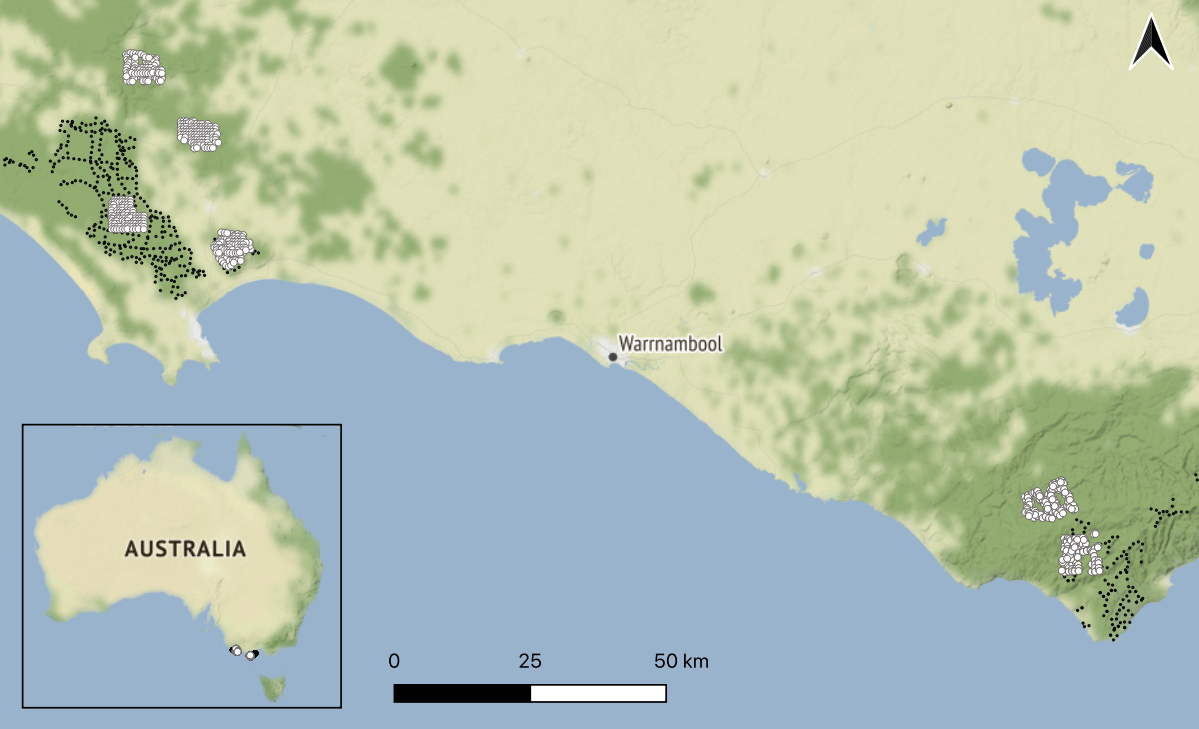
\includegraphics[width=1\linewidth]{figs/fig1} 

}

\caption{Locations of our eight study landscapes in south-west Victoria, Australia (red outlines). Note the two Lower Glenelg National Park landscapes in the far west are shown as one but are separated by a river. Locations of fox poison-bait stations are denoted by black dots. The Glenelg region is to the west and Otway region to the east. Native vegetation is indicated by dark green, with hill shading. \textit{Map tiles by Stamen Design, under CC BY 3.0, map data by OpenStreetMap, under CC BY SA.}}\label{fig:density-map}
\end{figure}

\newpage

\hypertarget{results}{%
\section{RESULTS}\label{results}}

\hypertarget{fox-occurrence}{%
\subsection{Fox occurrence}\label{fox-occurrence}}

In the Glenelg region, there was a clear difference in fox occurrence between paired impact (poison-baited) and non-impact landscapes for replicates 1 and 3, but only a marginal difference for replicate 2 (Fig. \ref{fig:foxplot}). In the Otway region, fox occurrence increased by 22\% in the non-impact landscape, and decreased by 43\% in the impact landscape over the three years (occurrence probability averaged at each camera-trap in the landscape). Fox occurrence in the Otway region was generally lower than the Glenelg region, with less fine-scale spatial variation. For example, fox occurrence was predicted to be spatially consistent across the entire Otway region in 2018 (Fig. \ref{fig:foxplot}). Fox model summaries and spatial standard error estimates are presented in SI Section \ref{density-app-fox}.

\hypertarget{feral-cats-in-the-glenelg-region}{%
\subsection{Feral cats in the Glenelg region}\label{feral-cats-in-the-glenelg-region}}

Across the six landscapes in the Glenelg region, we recorded 251 cat detections from 32,232 camera-trap nights (Table \ref{tab:density-stats}). We were able to identify 64\% of cat detections to the individual level; a total of 67 cats (6 -- 13 individuals per landscape). The exponential detector function was supported over the half-normal function (Table \ref{tab:density-aic-g-1}). The null model was more strongly supported than models with vegetation impacts on cat density and/or linear time trends on \emph{g}\textsubscript{0} (Table \ref{tab:density-aic-g-2}).

At a fine spatial scale, the model with a linear relationship between fox occurrence and cat density was strongly supported (AIC\textsubscript{c} 2.76 better than the null; Table \ref{tab:density-aic-g-3}). It indicated that cat density declined as fox occurrence increased (-0.32; 95\% CI: -0.57 - -0.07; Fig. \ref{fig:dcor}). There was no evidence of an impact of fox occurrence on cat detectability (Table \ref{tab:density-aic-g-3}). Regression splines added additional model parameters without changing predictions (Fig. \ref{fig:dcor}), and so, all nonlinear models ranked below their linear counterparts (Table \ref{tab:density-aic-g-3}).

Our hypothesis that cat density would be higher in landscapes with fox control was supported for the first and third replicate pairs: estimated cat densities were 2.5 (95\% CI: 1.5 - 4.2) and 3.7 (95\% CI: 1.4 - 9.5) times higher in the impact landscape than the paired non-impact landscape, respectively (Fig. \ref{fig:diffg}). For the second landscape pair, however, the estimated difference was positive but negligible (1.1; 95\% CI: 0.69 - 1.69). At the landscape level, there was some evidence that cat detectability was affected by fox occurrence; however the AIC\textsubscript{c} score was only 0.95 units better than the constant detectability model (Table \ref{tab:density-aic-g-4}) and the estimated effects were weak with high uncertainty. The detectability of cats in their activity centre (\emph{g}\textsubscript{0}) tended to increase with the probability of fox occurrence (0.24; 95\% CI: -0.32 - 0.80), as did sigma (0.13; 95\% CI: -0.14 - 0.41).

\hypertarget{feral-cats-in-the-otway-region}{%
\subsection{Feral cats in the Otway region}\label{feral-cats-in-the-otway-region}}

In the Otway region, we recorded 970 cat detections from 36,272 camera-trap nights (Table \ref{tab:density-stats}). We were able to identify 53\% of cat detections to the individual level; a total of 93 cats (20 -- 30 individuals per landscape). The exponential detector function was strongly supported over the half-normal function (Table \ref{tab:density-aic-o-1}). The null model was more strongly supported than the models with vegetation impacts on cat density and/or linear time trends on \emph{g}\textsubscript{0} (Table \ref{tab:density-aic-o-2}).

There was some evidence that cat density was negatively correlated with fox occurrence at a fine spatial scale: the two top-ranked models included a linear and a non-linear effect of fox occurrence on cat density, respectively; however, a model without a fox occurrence term received similar support (dAIC\textsubscript{c} = 0.80; Table \ref{tab:density-aic-o-3}). The 95\% confidence interval around the linear coefficient from the top-ranked model marginally overlapped zero (-0.26; 95\% CI: -0.55 - 0.02) indicating that cat density declined as fox occurrence increased in the Otways at a similar rate to Glenelg, but with slightly greater uncertainty (Fig. \ref{fig:dcor}). However, the equivalent nonlinear model predicted that cat density only declined (at a steeper rate) in the mid-high range of fox occurrence probability (Fig. \ref{fig:dcor}). Equivalent pairs of linear model and nonlinear models were indistinguishable based on AIC\textsubscript{c} scores (Table \ref{tab:density-aic-o-3}).
There was also strong support for an effect of fox occurrence on cat detectability at a fine spatial scale (Fig. \ref{fig:detcor}; Table \ref{tab:density-aic-o-4}). Where fox occurrence was higher, cats were less detectable in their activity centres (i.e., negative association with \emph{g}\textsubscript{0}; -0.69; 95\% CI: -1.11 - -0.27; Fig. \ref{fig:detcor}A) and ranged further (i.e., positive association with sigma; coefficient 0.30; 95\% CI: 0.13 - 0.47; Fig. \ref{fig:detcor}B). The equivalent nonlinear model predicted detectability changes to have occurred only in the low-mid range of fox occurrence (Fig. \ref{fig:detcor}).

Our hypothesis that cat density in the impact landscape would increase relative to the non-impact landscape with fox control was supported, however there was considerable uncertainty. Cat density tended to be lower in the impact than non-impact landscape prior to fox-baiting (i.e., in 2017), although the confidence intervals for the two density estimates overlapped substantially (Fig. \ref{fig:diffo}). In 2018, cat density decreased in the non-impact landscape and increased in the impact landscape, converging to near-identical density estimates. These patterns continued into 2019, with cat density now somewhat higher in the impact landscape than non-impact landscape. Overlap in the response ratio confidence intervals for successive years was high, but the comparison between 2017 to 2019 suggests a meaningful increase in cat density at the impact landscape relative to the non-impact landscape (Fig. \ref{fig:diffo}B). Like the fine scale model, there was strong evidence that cat detectability was impacted by fox occurrence (Table \ref{tab:density-aic-o-4}).

\newpage

\begin{figure}

{\centering \includegraphics[width=1\linewidth]{figs/fig2_600dpi} 

}

\caption{Predicted red fox \textit{Vulpes vulpes} occurrence derived from generalised additive models within each impact (I) and paired non-impact (NI) landscape in the Glenelg (a) and Otway (b) regions, Australia. Predicted fox occurrence was used as a predictor of feral cat Felis catus density in the spatial mark-resight models.}\label{fig:foxplot}
\end{figure}

\newpage

\begin{figure}

{\centering \includegraphics[width=1\linewidth]{figs/foxD_600dpi} 

}

\caption{Linear (solid lines) and nonlinear (dashed lines) models predicted that feral cat \textit{Felis catus} density increased with declining probability of red fox \textit{Vulpes vulpes} occurrence (log-transformed) in the Glenelg and Otway regions, Australia. Shaded areas indicate 95\% confidence intervals.}\label{fig:dcor}
\end{figure}

\newpage

\begin{figure}

{\centering \includegraphics[width=1\linewidth]{figs/foxDet_otways_600dpi} 

}

\caption{Linear (solid lines) and nonlinear (dashed lines) models of feral cat \textit{Felis catus} detectability as a function of log-transformed red fox \textit{Vulpes vulpes} occurrence in the Otway Ranges, Australia. The probability of detecting a feral cat in its activity centre per 24-hour occasion (\textit{g}\textsubscript{0}) decreased with the probability of fox occurrence (a), while sigma (which is related to home range size; exponential units) increased (b). Shaded areas indicate 95\% confidence intervals.}\label{fig:detcor}
\end{figure}

\newpage

\begin{figure}

{\centering \includegraphics[width=1\linewidth]{figs/glenelg_estimates_600dpi} 

}

\caption{Landscape-scale feral cat \textit{Felis catus} density estimates (a) and response ratio of cat density in the impact landscape relative to the paired non-impact landscape for each replicate (b) in the Glenelg region, Australia. Poison-baiting for foxes \textit{Vulpes vulpes} has been conducted in the impact landscapes for more than 13 years. Grey dashed line represents no difference between the paired landscapes. Error bars represent 95\% confidence intervals.}\label{fig:diffg}
\end{figure}

\newpage

\begin{figure}

{\centering \includegraphics[width=1\linewidth]{figs/otways_estimates_600dpi} 

}

\caption{Landscape-scale feral cat \textit{Felis catus} density estimates (a) and response ratio of cat density in the impact landscape relative to the non-impact landscape for each survey year (b) in the Otway region, Australia. In 2017, surveys were conducted approximately two months before lethal red fox \textit{Vulpes vulpes} control commenced in the impact landscape; control lapsed for six months prior to the 2018 survey. Error bars represent 95\% confidence intervals. Overlap with the grey dashed line in (b) represents no difference in density between the paired landscapes for that year; the proportion overlap between response ratio confidence intervals across years provides evidence for a change in difference.}\label{fig:diffo}
\end{figure}

\newpage

\hypertarget{discussion}{%
\section{DISCUSSION}\label{discussion}}

Our study is one of the first to provide replicated, experimental evidence that apex predator suppression can increase mesopredator population density. Our study provides two lines of evidence that foxes can exert top-down control on feral cats in the forests of south-eastern Australia: feral cat density was (1) higher where fine-scale fox occurrence probability was lowest, and (2) commonly higher in landscapes where fox control occurred. This is alarming because targeted fox control is a widely used conservation strategy; this unintended consequence could dampen benefits to native prey and even further threaten these species. However, as our findings highlight, mesopredator release of cats following fox control is unlikely to occur universally; the degree of fox suppression varies and fox-cat interactions are likely to be context and scale-dependent. More broadly, our study illustrates how correlative and experimental approaches provide complementary lines of evidence when investigating interactions between predator species, and the importance of disentangling changes in population density from changes in detectability.

We were able to exploit a gradient in fox occurrence caused by lethal control to investigate associations between cat density and fox occurrence at a fine spatial scale across two separate regions. At this scale, we observed a consistently negative association between cat density and fox occurrence, supporting our first hypothesis, although there was more uncertainty around the relationship in the Otway region. We acknowledge that it could also simply reflect differences in niche preference, rather than foxes excluding cats or cats avoiding foxes. However, we consider this unlikely given we observed the relationship across an artificial gradient of fox occurrence caused by lethal control.

There is contention around whether linear regression is appropriate for investigating correlations between different predator species, as subordinate predators may only be suppressed when apex predator abundance is high (Johnson \& VanDerWal 2009). We found no evidence of non-linear associations between foxes and cats in the Glenelg region, while linear and non-linear models performed equally well in the Otway region. Non-linear models in the Otway region predicted that cat density declined only in the mid-high range of fox occurrence, while behavioural changes were seen in the low-mid range of fox occurrence. Perhaps cats can successfully avoid foxes through behavioural change where foxes are rare, but this is ineffective where foxes are common. This could explain the lack of evidence for foxes impacting cat detectability in the Glenelg region where fox occupancy is relatively high. Alternatively, behavioural changes may be untenable for cats in the Glenelg region because small mammal abundance is relatively low and fox avoidance strategies likely come at the expense of hunting success (Sih 1980; Wilson \emph{et al.} 2010).

Where fox occurrence was higher in the Otway Ranges, cats were less detectable in their activity centres and ranged further (Fig. \ref{fig:detcor}). Low detectability is likely to correlate with fewer apex predator encounters, and has been observed in other predator interaction studies (e.g.~Lombardi \emph{et al.} 2017). An increase in cat ranging behaviour (sigma) with fox control supports observations made by Molsher \emph{et al.} (2017), and may reflect a direct avoidance strategy. Animal movement rates are expected to increase in response to unpredictable threats (Riotte-Lambert \& Matthiopoulos 2020). Alternatively, cats may consider foxes predictable and avoid locations they frequent, thus having to range further to obtain the same amount of food resources. In a similar forest habitat, Buckmaster (2012) observed large `holes' in the home range of each GPS-collared cat; they confirmed that this was not due to an absence of prey and hypothesised that it could be due to apex predator avoidance. Regardless of the cause, variation in mesopredator detectability and movement rates with apex predator populations has serious implications for the interpretation of studies that compare relative abundance indices and spatial overlap of predator species without disentangling behaviour and detectability from density (Efford \& Dawson 2012; Neilson \emph{et al.} 2018; Stewart \emph{et al.} 2018; Broadley \emph{et al.} 2019).

In the Glenelg region where fox-baiting had occurred for more than 13 years, feral cat density was considerably higher in two out of three distinct landscapes than in similar, unbaited landscapes. The outlier is most likely due to limited suppression of foxes at Mt Clay despite ongoing fox control (Fig. \ref{fig:foxplot}). Mt Clay is a small forest block surrounded entirely by unbaited farmland. Simulation modelling indicates that the size of the baited area is a key driver of the degree of reduction in the fox population (Hradsky \emph{et al.} 2019; Francis, Robley, \& Hradsky 2020). Studies of fox-cat (and other predator-predator) interactions often use the presence of a management program as a proxy for lower apex predator abundance and distribution (e.g.~Hunter \emph{et al.} 2018). Our findings strongly indicate the need to directly measure the apex predator population in order to reliably interpret the responses of subordinate species (Salo \emph{et al.} 2010).

In the Otway region, we observed a weaker--but increasing--effect of fox control on cat density, to be expected from a recently commenced and less intensive fox-baiting program. The short duration of baiting in the Otway region may mean that changes in adult cat density are yet to fully manifest as foxes potentially suppress cats by reducing recruitment rates. Cats may also respond to an increase in shared prey availability following fox suppression (Stobo-Wilson \emph{et al.} 2020). A time-lagged release of cats following fox control would explain eruptions and subsequent crashes commonly observed in shared mammalian prey populations two to ten years following fox control commencement (Duncan \emph{et al.} 2020). Alternatively, top-down suppression by foxes and competition may be weaker in this highly productive environment where prey abundance was relatively high, fox occurrence was already relatively low, and overall cat densities were consistently high (Johnson \& VanDerWal 2009; Greenville \emph{et al.} 2014; Newsome \emph{et al.} 2017). Our surveys provide important baselines against which to compare future changes in predator populations as the fox-baiting program continues.

Our study is among the very few which have used a direct measure of density to test mesopredator release. Previous studies have mostly used live capture-rates to infer population density, without accounting for behavioural or detectability changes (e.g.~Arjo \emph{et al.} 2007; Karki, Gese, \& Klavetter 2007; Thompson \& Gese 2007; Berger, Gese, \& Berger 2008; Jones, Van Vuren, \& Crooks 2008). Contention about mesopredator release has centred on such methods (Hayward \emph{et al.} 2015); as well as unaccounted species interactions in complex predator guilds (Levi \& Wilmers 2012; Jachowski \emph{et al.} 2020). In contrast, our study tests the mesopredator release theory using a combined behavioural and numerical approach, in a system with a simplified carnivore guild. One limitation of our approach is that uncertainty from our fox occurrence models was not propagated into the spatial mark-resight models. A full Bayesian integration of the fox occurrence analysis and the spatial mark-resight model to address this is not yet implemented. The development of open population spatial mark-resight models would also improve parameter estimates for multi-season surveys.

The results of our study may explain why pest management that only targets foxes--one of the most prevalent conservation actions in Australia--does not consistently improve native prey persistence (Dexter \& Murray 2009; Robley \emph{et al.} 2014; Lindenmayer \emph{et al.} 2018; Duncan \emph{et al.} 2020; Wayne \emph{et al.} 2017). More evidence is required to understand the circumstances in which lethal fox control increases cat density, particularly the role of baseline fox and prey densities. A more integrated approach to invasive predator management, where foxes and cats are simultaneously or otherwise optimally controlled could substantially improve biodiversity outcomes (Risbey \emph{et al.} 2000; Comer \emph{et al.} 2020). If this is not feasible, changes in invasive mesopredator density and the outcomes for native prey species should be closely monitored as part of any control program for invasive apex predators, with triggers for ceasing apex predator control or commencing integrated management if single-species control proves counterproductive for the conservation of threatened prey species.

\newpage

\hypertarget{acknowledgements}{%
\section*{ACKNOWLEDGEMENTS}\label{acknowledgements}}
\addcontentsline{toc}{section}{ACKNOWLEDGEMENTS}

We acknowledge and pay respect to the Gadubanud and Gunditjmara peoples on whose traditional lands this study took place. Surveys were conducted under University of Melbourne Animal Ethics Committee approval 1714119 and Victorian Government Department of Environment, Land Water and Planning Research Permit 10008273. This experiment was conducted in cooperation with the Glenelg Ark (Department of Environment, Land Water and Planning) and Otway Ark (Parks Victoria) working groups. Ethan Le Duc, Michael Murrell, Dylan Thomas, Rhys Weber, Chris Johansson, Lachlan Levings and Liz Beever carried out the Lower Glenelg National Park surveys, with Luke Woodford identifying cats. We are extremely grateful to our field assistants: Shauni Omond, Shayne Neal, Asitha Samarawickrama, Shelley Thompson, Erin Harris, Hannah Killian, Lani Watson, Mark Dorman, Jack Davis,Carl Roffey, Bruce Edley, Larissa Oliveira Gonçalves, Ben Lake, Chantelle Geissler, Aviya Naccarella, Emily Gronow, Harley England, David Pitts, Annie Hobby, Louise Falls, Thomas McKinnon, Jimmy Downie, Marney Hradsky, Stephanie Samson, Robin Sinclair, Asmaa Alhusainan, Kelly Forrester, Tammana Wadawani, Emily McColl-Gausden, Emily Gregg, Hannah Edwards, Adam Beck, Vishnu Memnon, Sandy Lu, Dr Pia Lentini, Prof.~Nick Golding, Emily McColl-Gausden, Nina Page, Maggie Campbell-Jones, Kyle Quinn and Jack Dickson. This manuscript was improved by comments from William Geary; Dr Joanne Potts also gave instrumental advice on fitting spatial mark-resight models. Our study was generously supported by the Conservation Ecology Centre, the Victorian Government Department of Environment, Land Water and Planning, Arthur Rylah Institute for Environmental Research, Parks Victoria, the Australian Government's National Environmental Science Program through the Threatened Species Recovery Hub, and ARC Linkage Project LP170101134. M.W.R also receives support from an Australian Government Research Training Program Scholarship.

\newpage

\hypertarget{references}{%
\section*{REFERENCES}\label{references}}
\addcontentsline{toc}{section}{REFERENCES}

\hypertarget{refs}{}
\leavevmode\hypertarget{ref-alston2019reciprocity}{}%
Alston, J., Maitland, B., Brito, B., Esmaeili, S., Ford, A., Hays, B., Jesmer, B., Molina, F. \& Goheen, J. (2019) Reciprocity in restoration ecology: When might large carnivore reintroduction restore ecosystems? \emph{Biological conservation}, \textbf{234}, 82--89.

\leavevmode\hypertarget{ref-arjo2007changes}{}%
Arjo, W.M., Gese, E.M., Bennett, T.J. \& Kozlowski, A.J. (2007) Changes in kit fox--coyote--prey relationships in the Great Basin Desert, Utah. \emph{Western North American Naturalist}, \textbf{67}, 389--401.

\leavevmode\hypertarget{ref-ballari2016potential}{}%
Ballari, S.A., Kuebbing, S.E. \& Nuñez, M.A. (2016) Potential problems of removing one invasive species at a time: A meta-analysis of the interactions between invasive vertebrates and unexpected effects of removal programs. \emph{PeerJ}, \textbf{4}, e2029.

\leavevmode\hypertarget{ref-berger2008indirect}{}%
Berger, K.M., Gese, E.M. \& Berger, J. (2008) Indirect effects and traditional trophic cascades: A test involving wolves, coyotes, and pronghorn. \emph{Ecology}, \textbf{89}, 818--828.

\leavevmode\hypertarget{ref-bode2015eradicating}{}%
Bode, M., Baker, C.M. \& Plein, M. (2015) Eradicating down the food chain: Optimal multispecies eradication schedules for a commonly encountered invaded island ecosystem. \emph{Journal of Applied Ecology}, \textbf{52}, 571--579.

\leavevmode\hypertarget{ref-borchers2008spatially}{}%
Borchers, D.L. \& Efford, M.G. (2008) Spatially explicit maximum likelihood methods for capture--recapture studies. \emph{Biometrics}, \textbf{64}, 377--385.

\leavevmode\hypertarget{ref-broadley2019density}{}%
Broadley, K., Burton, A.C., Avgar, T. \& Boutin, S. (2019) Density-dependent space use affects interpretation of camera trap detection rates. \emph{Ecology and evolution}, \textbf{9}, 14031--14041.

\leavevmode\hypertarget{ref-buckmaster2012ecology}{}%
Buckmaster, A.J. (2012) \emph{Ecology of the Feral Cat \textup{(Felis catus)} in the Tall Forests of Far East Gippsland}. PhD thesis, University of Sydney.; School of Biological Sciences; University of Sydney.; School of Biological Sciences.

\leavevmode\hypertarget{ref-BOM2021}{}%
Bureau of Meteorology. (2021) Climate data online.

\leavevmode\hypertarget{ref-burnham2004multimodel}{}%
Burnham, K.P. \& Anderson, D.R. (2004) Multimodel inference: Understanding AIC and BIC in model selection. \emph{Sociological methods \& research}, \textbf{33}, 261--304.

\leavevmode\hypertarget{ref-chandler2013spatially}{}%
Chandler, R.B. \& Royle, J.A. (2013) Spatially explicit models for inference about density in unmarked or partially marked populations. \emph{The Annals of Applied Statistics}, \textbf{7}, 936--954.

\leavevmode\hypertarget{ref-christie2019simple}{}%
Christie, A.P., Amano, T., Martin, P.A., Shackelford, G.E., Simmons, B.I. \& Sutherland, W.J. (2019) Simple study designs in ecology produce inaccurate estimates of biodiversity responses. \emph{Journal of Applied Ecology}, \textbf{56}, 2742--2754.

\leavevmode\hypertarget{ref-claridge2010trends}{}%
Claridge, A.W., Cunningham, R.B., Catling, P.C. \& Reid, A.M. (2010) Trends in the activity levels of forest-dwelling vertebrate fauna against a background of intensive baiting for foxes. \emph{Forest Ecology and Management}, \textbf{260}, 822--832.

\leavevmode\hypertarget{ref-comer2020integrating}{}%
Comer, S., Clausen, L., Cowen, S., Pinder, J., Thomas, A., Burbidge, A.H., Tiller, C., Algar, D. \& Speldewinde, P. (2020) Integrating feral cat (felis catus) control into landscape-scale introduced predator management to improve conservation prospects for threatened fauna: A case study from the south coast of Western Australia. \emph{Wildlife Research}, \textbf{47}, 762--778.

\leavevmode\hypertarget{ref-courchamp1999cats}{}%
Courchamp, F., Langlais, M. \& Sugihara, G. (1999) Cats protecting birds: Modelling the mesopredator release effect. \emph{Journal of Animal Ecology}, \textbf{68}, 282--292.

\leavevmode\hypertarget{ref-crooks1999mesopredator}{}%
Crooks, K.R. \& Soulé, M.E. (1999) Mesopredator release and avifaunal extinctions in a fragmented system. \emph{Nature}, \textbf{400}, 563--566.

\leavevmode\hypertarget{ref-cumming2005inference}{}%
Cumming, G. \& Finch, S. (2005) Inference by eye: Confidence intervals and how to read pictures of data. \emph{American psychologist}, \textbf{60}, 170.

\leavevmode\hypertarget{ref-davey2006exotic}{}%
Davey, C., Sinclair, A., Pech, R.P., Arthur, A.D., Krebs, C.J., Newsome, A., Hik, D., Molsher, R. \& Allcock, K. (2006) Do exotic vertebrates structure the biota of Australia? An experimental test in new south wales. \emph{Ecosystems}, \textbf{9}, 992--1008.

\leavevmode\hypertarget{ref-dexter2009impact}{}%
Dexter, N. \& Murray, A. (2009) The impact of fox control on the relative abundance of forest mammals in east gippsland, victoria. \emph{Wildlife Research}, \textbf{36}, 252--261.

\leavevmode\hypertarget{ref-doherty2017stop}{}%
Doherty, T.S. \& Ritchie, E.G. (2017) Stop jumping the gun: A call for evidence-based invasive predator management. \emph{Conservation Letters}, \textbf{10}, 15--22.

\leavevmode\hypertarget{ref-duncan2020eruptive}{}%
Duncan, R.P., Dexter, N., Wayne, A. \& Hone, J. (2020) Eruptive dynamics are common in managed mammal populations. \emph{Ecology}, \textbf{101}, e03175.

\leavevmode\hypertarget{ref-efford2021secr}{}%
Efford, M.G. (2021) Secr: Spatially explicit capture-recapture models. R package version 4.4.4, \url{http://CRAN.R-project.org/package=secr}

\leavevmode\hypertarget{ref-efford2012occupancy}{}%
Efford, M.G. \& Dawson, D.K. (2012) Occupancy in continuous habitat. \emph{Ecosphere}, \textbf{3}, 1--15.

\leavevmode\hypertarget{ref-efford2014compensatory}{}%
Efford, M.G. \& Mowat, G. (2014) Compensatory heterogeneity in spatially explicit capture--recapture data. \emph{Ecology}, \textbf{95}, 1341--1348.

\leavevmode\hypertarget{ref-elmhagen2007trophic}{}%
Elmhagen, B. \& Rushton, S.P. (2007) Trophic control of mesopredators in terrestrial ecosystems: Top-down or bottom-up? \emph{Ecology Letters}, \textbf{10}, 197--206.

\leavevmode\hypertarget{ref-finke2004predator}{}%
Finke, D.L. \& Denno, R.F. (2004) Predator diversity dampens trophic cascades. \emph{Nature}, \textbf{429}, 407--410.

\leavevmode\hypertarget{ref-fisher2015cat}{}%
Fisher, P., Algar, D., Murphy, E., Johnston, M. \& Eason, C. (2015) How does cat behaviour influence the development and implementation of monitoring techniques and lethal control methods for feral cats? \emph{Applied Animal Behaviour Science}, \textbf{173}, 88--96.

\leavevmode\hypertarget{ref-francis2020evaluating}{}%
Francis, L., Robley, A. \& Hradsky, B. (2020) \emph{Evaluating Fox Management Strategies Using a Spatially Explicit Population}. Arthur Rylah Institute for Environmental Research Technical Report Series No. 304. Department of Environment, Land, Water; Planning, Heidelberg, Victoria.

\leavevmode\hypertarget{ref-glen2005complex}{}%
Glen, A.S. \& Dickman, C.R. (2005) Complex interactions among mammalian carnivores in Australia, and their implications for wildlife management. \emph{Biological reviews}, \textbf{80}, 387--401.

\leavevmode\hypertarget{ref-greenville2014bottom}{}%
Greenville, A.C., Wardle, G.M., Tamayo, B. \& Dickman, C.R. (2014) Bottom-up and top-down processes interact to modify intraguild interactions in resource-pulse environments. \emph{Oecologia}, \textbf{175}, 1349--1358.

\leavevmode\hypertarget{ref-hastings2001transient}{}%
Hastings, A. (2001) Transient dynamics and persistence of ecological systems. \emph{Ecology Letters}, \textbf{4}, 215--220.

\leavevmode\hypertarget{ref-hayward2015ecologists}{}%
Hayward, M.W., Boitani, L., Burrows, N.D., Funston, P.J., Karanth, K.U., MacKenzie, D.I., Pollock, K.H. \& Yarnell, R.W. (2015) Ecologists need robust survey designs, sampling and analytical methods. \emph{Journal of Applied Ecology}, \textbf{52}, 286--290.

\leavevmode\hypertarget{ref-hradsky2019foxnet}{}%
Hradsky, B.A., Kelly, L.T., Robley, A. \& Wintle, B.A. (2019) FoxNet: An individual-based model framework to support management of an invasive predator, the red fox. \emph{Journal of Applied Ecology}, \textbf{56}, 1460--1470.

\leavevmode\hypertarget{ref-hradsky2017human}{}%
Hradsky, B.A., Robley, A., Alexander, R., Ritchie, E.G., York, A. \& Di Stefano, J. (2017) Human-modified habitats facilitate forest-dwelling populations of an invasive predator, \emph{(Vulpes vulpes)}. \emph{Scientific Reports}, \textbf{7}, 1--12.

\leavevmode\hypertarget{ref-hunter2018not}{}%
Hunter, D.O., Lagisz, M., Leo, V., Nakagawa, S. \& Letnic, M. (2018) Not all predators are equal: A continent-scale analysis of the effects of predator control on Australian mammals. \emph{Mammal Review}, \textbf{48}, 108--122.

\leavevmode\hypertarget{ref-jachowski2020identifying}{}%
Jachowski, D.S., Butler, A., Eng, R.Y.Y., Gigliotti, L., Harris, S. \& Williams, A. (2020) Identifying mesopredator release in multi-predator systems: A review of evidence from north america. \emph{Mammal Review}, \textbf{50}, 367--381.

\leavevmode\hypertarget{ref-jackson2015interactions}{}%
Jackson, M.C. (2015) Interactions among multiple invasive animals. \emph{Ecology}, \textbf{96}, 2035--2041.

\leavevmode\hypertarget{ref-johnson2009evidence}{}%
Johnson, C.N. \& VanDerWal, J. (2009) Evidence that dingoes limit abundance of a mesopredator in eastern Australian forests. \emph{Journal of Applied Ecology}, \textbf{46}, 641--646.

\leavevmode\hypertarget{ref-jones2008sudden}{}%
Jones, K.L., Van Vuren, D.H. \& Crooks, K.R. (2008) Sudden Increase in a Rare Endemic Carnivore: Ecology of the Island Spotted Skunk. \emph{Journal of Mammalogy}, \textbf{89}, 75--86.

\leavevmode\hypertarget{ref-karki2007effects}{}%
Karki, S.M., Gese, E.M. \& Klavetter, M.L. (2007) Effects of coyote population reduction on swift fox demographics in southeastern colorado. \emph{The Journal of Wildlife Management}, \textbf{71}, 2707--2718.

\leavevmode\hypertarget{ref-kuebbing2015negative}{}%
Kuebbing, S.E. \& Nuñez, M.A. (2015) Negative, neutral, and positive interactions among nonnative plants: Patterns, processes, and management implications. \emph{Global Change Biology}, \textbf{21}, 926--934.

\leavevmode\hypertarget{ref-lazenby2015effects}{}%
Lazenby, B.T., Mooney, N.J. \& Dickman, C.R. (2015) Effects of low-level culling of feral cats in open populations: A case study from the forests of southern tasmania. \emph{Wildlife Research}, \textbf{41}, 407--420.

\leavevmode\hypertarget{ref-legge2020cat}{}%
Legge, S., Taggart, P.L., Dickman, C.R., Read, J.L. \& Woinarski, J.C. (2020) \emph{Wildlife Research}, \textbf{47}, 731--746.

\leavevmode\hypertarget{ref-levi2012wolves}{}%
Levi, T. \& Wilmers, C.C. (2012) Wolves--coyotes--foxes: A cascade among carnivores. \emph{Ecology}, \textbf{93}, 921--929.

\leavevmode\hypertarget{ref-lindenmayer2018conservation}{}%
Lindenmayer, D.B., Wood, J., MacGregor, C., Foster, C., Scheele, B., Tulloch, A., Barton, P., Banks, S., Robinson, N., Dexter, N., O'Loughlin, L.S. \& Legge, S. (2018) Conservation conundrums and the challenges of managing unexplained declines of multiple species. \emph{Biological Conservation}, \textbf{221}, 279--292.

\leavevmode\hypertarget{ref-lombardi2017coyote}{}%
Lombardi, J.V., Comer, C.E., Scognamillo, D.G. \& Conway, W.C. (2017) Coyote, fox, and bobcat response to anthropogenic and natural landscape features in a small urban area. \emph{Urban Ecosystems}, \textbf{20}, 1239--1248.

\leavevmode\hypertarget{ref-marlow2015cats}{}%
Marlow, N.J., Thomas, N.D., Williams, A.A., Macmahon, B., Lawson, J., Hitchen, Y., Angus, J. \& Berry, O. (2015) Cats \emph{(Felis catus)} are more abundant and are the dominant predator of woylies (bettongia penicillata) after sustained fox \emph{(Vulpes vulpes)} control. \emph{Australian Journal of Zoology}, \textbf{63}, 18--27.

\leavevmode\hypertarget{ref-mcleod2014fertility}{}%
McLeod, S.R. \& Saunders, G. (2014) Fertility control is much less effective than lethal baiting for controlling foxes. \emph{Ecological Modelling}, \textbf{273}, 1--10.

\leavevmode\hypertarget{ref-medina2011global}{}%
Medina, F.M., Bonnaud, E., Vidal, E., Tershy, B.R., Zavaleta, E.S., Josh Donlan, C., Keitt, B.S., Le Corre, M., Horwath, S.V. \& Nogales, M. (2011) A global review of the impacts of invasive cats on island endangered vertebrates. \emph{Global Change Biology}, \textbf{17}, 3503--3510.

\leavevmode\hypertarget{ref-miller2014finite}{}%
Miller, D.L. \& Wood, S.N. (2014) Finite area smoothing with generalized distance splines. \emph{Environmental and ecological statistics}, \textbf{21}, 715--731.

\leavevmode\hypertarget{ref-molsher2017mesopredator}{}%
Molsher, R., Newsome, A.E., Newsome, T.M. \& Dickman, C.R. (2017) Mesopredator management: Effects of red fox control on the abundance, diet and use of space by feral cats. \emph{PLoS One}, \textbf{12}, e0168460.

\leavevmode\hypertarget{ref-moseby2019understanding}{}%
Moseby, K.E., Letnic, M., Blumstein, D.T. \& West, R. (2019) Understanding predator densities for successful co-existence of alien predators and threatened prey. \emph{Austral Ecology}, \textbf{44}, 409--419.

\leavevmode\hypertarget{ref-moseby2020effectiveness}{}%
Moseby, K., McGregor, H. \& Read, J. (2020) Effectiveness of the felixer grooming trap for the control of feral cats: A field trial in arid South Australia. \emph{Wildlife Research}, \textbf{47}, 599--609.

\leavevmode\hypertarget{ref-neilson2018animal}{}%
Neilson, E.W., Avgar, T., Burton, A.C., Broadley, K. \& Boutin, S. (2018) Animal movement affects interpretation of occupancy models from camera-trap surveys of unmarked animals. \emph{Ecosphere}, \textbf{9}, e02092.

\leavevmode\hypertarget{ref-newsome2017top}{}%
Newsome, T.M., Greenville, A.C., Ćirović, D., Dickman, C.R., Johnson, C.N., Krofel, M., Letnic, M., Ripple, W.J., Ritchie, E.G., Stoyanov, S. \& others. (2017) Top predators constrain mesopredator distributions. \emph{Nature communications}, \textbf{8}, 1--7.

\leavevmode\hypertarget{ref-rayner2007spatial}{}%
Rayner, M.J., Hauber, M.E., Imber, M.J., Stamp, R.K. \& Clout, M.N. (2007) Spatial heterogeneity of mesopredator release within an oceanic island system. \emph{Proceedings of the National Academy of Sciences}, \textbf{104}, 20862--20865.

\leavevmode\hypertarget{ref-reddiex2007control}{}%
Reddiex, B., Forsyth, D.M., McDonald-Madden, E., Einoder, L.D., Griffioen, P.A., Chick, R.R. \& Robley, A.J. (2007) Control of pest mammals for biodiversity protection in Australia. I. Patterns of control and monitoring. \emph{Wildlife Research}, \textbf{33}, 691--709.

\leavevmode\hypertarget{ref-riley1999index}{}%
Riley, S.J., DeGloria, S.D. \& Elliot, R. (1999) Index that quantifies topographic heterogeneity. \emph{intermountain Journal of sciences}, \textbf{5}, 23--27.

\leavevmode\hypertarget{ref-riotte-lambert2020environmental}{}%
Riotte-Lambert, L. \& Matthiopoulos, J. (2020) Environmental predictability as a cause and consequence of animal movement. \emph{Trends in Ecology \& Evolution}, \textbf{35}, 163--174.

\leavevmode\hypertarget{ref-risbey2000impacts}{}%
Risbey, D.A., Calver, M.C., Short, J., Bradley, J.S. \& Wright, I.W. (2000) The impact of cats and foxes on the small vertebrate fauna of Heirisson Prong, Western Australia. II. A field experiment. \emph{Wildlife Research}, \textbf{27}, 223--235.

\leavevmode\hypertarget{ref-robley2014long}{}%
Robley, A., Gormley, A.M., Forsyth, D.M. \& Triggs, B. (2014) Long-term and large-scale control of the introduced red fox increases native mammal occupancy in Australian forests. \emph{Biological Conservation}, \textbf{180}, 262--269.

\leavevmode\hypertarget{ref-rogan2019influence}{}%
Rogan, M.S., Balme, G.A., Distiller, G., Pitman, R.T., Broadfield, J., Mann, G.K., Whittington-Jones, G.M., Thomas, L.H. \& O'Riain, M.J. (2019) The influence of movement on the occupancy--density relationship at small spatial scales. \emph{Ecosphere}, \textbf{10}, e02807.

\leavevmode\hypertarget{ref-ruscoe2011unexpected}{}%
Ruscoe, W.A., Ramsey, D.S., Pech, R.P., Sweetapple, P.J., Yockney, I., Barron, M.C., Perry, M., Nugent, G., Carran, R., Warne, R. \& others. (2011) Unexpected consequences of control: Competitive vs. Predator release in a four-species assemblage of invasive mammals. \emph{Ecology Letters}, \textbf{14}, 1035--1042.

\leavevmode\hypertarget{ref-salo2010predator}{}%
Salo, P., Banks, P.B., Dickman, C.R. \& Korpimäki, E. (2010) Predator manipulation experiments: Impacts on populations of terrestrial vertebrate prey. \emph{Ecological Monographs}, \textbf{80}, 531--546.

\leavevmode\hypertarget{ref-sih1980optimal}{}%
Sih, A. (1980) Optimal behavior: Can foragers balance two conflicting demands? \emph{Science}, \textbf{210}, 1041--1043.

\leavevmode\hypertarget{ref-smith2020zooming}{}%
Smith, J.A., Suraci, J.P., Hunter, J.S., Gaynor, K.M., Keller, C.B., Palmer, M.S., Atkins, J.L., Castañeda, I., Cherry, M.J., Garvey, P.M. \& others. (2020) Zooming in on mechanistic predator--prey ecology: Integrating camera traps with experimental methods to reveal the drivers of ecological interactions. \emph{Journal of Animal Ecology}, \textbf{89}, 1997--2012.

\leavevmode\hypertarget{ref-soule1988reconstructed}{}%
Soulé, M.E., Bolger, D.T., Alberts, A.C., Wrights, J., Sorice, M. \& Hill, S. (1988) Reconstructed dynamics of rapid extinctions of chaparral-requiring birds in urban habitat islands. \emph{Conservation Biology}, \textbf{2}, 75--92.

\leavevmode\hypertarget{ref-stephens2015management}{}%
Stephens, P.A., Pettorelli, N., Barlow, J., Whittingham, M.J. \& Cadotte, M.W. (2015) Management by proxy? The use of indices in applied ecology. \emph{Journal of Applied Ecology}, \textbf{52}, 1--6.

\leavevmode\hypertarget{ref-stewart2018species}{}%
Stewart, F.E.C., Fisher, J.T., Burton, A.C. \& Volpe, J.P. (2018) Species occurrence data reflect the magnitude of animal movements better than the proximity of animal space use. \emph{Ecosphere}, \textbf{9}, e02112.

\leavevmode\hypertarget{ref-stobo2020management}{}%
Stobo-Wilson, A.M., Brandle, R., Johnson, C.N. \& Jones, M.E. (2020) Management of invasive mesopredators in the Flinders Ranges, South Australia: Effectiveness and implications. \emph{Wildlife Research}, \textbf{47}, 720--730.

\leavevmode\hypertarget{ref-stobo2021sharing}{}%
Stobo-Wilson, A.M., Murphy, B.P., Crawford, H.M., Dawson, S.J., Dickman, C.R., Doherty, T.S., Fleming, P.A., Gentle, M.N., Legge, S.M., Newsome, T.M., Palmer, R., Rees, M.W., Ritchie, E.G., Speed, J., Stuart, J.-M., Thompson, E., Turpin, J. \& Woinarski, J.C.Z. (2021a) Sharing meals: Predation on Australian mammals by the introduced european red fox compounds and complements predation by feral cats. \emph{Biological Conservation}, \textbf{261}, 109284.

\leavevmode\hypertarget{ref-stobo2021reptiles}{}%
Stobo-Wilson, A.M., Murphy, B.P., Legge, S.M., Chapple, D.G., Crawford, H.M., Dawson, S.J., Dickman, C.R., Doherty, T.S., Fleming, P.A., Gentle, M. \& others. (2021b) Reptiles as food: Predation of Australian reptiles by introduced red foxes compounds and complements predation by cats. \emph{Wildlife Research}, \textbf{48}, 470--480.

\leavevmode\hypertarget{ref-thompson2007food}{}%
Thompson, C.M. \& Gese, E.M. (2007) Food webs and intraguild predation: Community interactions of a native mesocarnivore. \emph{Ecology}, \textbf{88}, 334--346.

\leavevmode\hypertarget{ref-towerton2011detecting}{}%
Towerton, A.L., Penman, T.D., Kavanagh, R.P. \& Dickman, C.R. (2011) Detecting pest and prey responses to fox control across the landscape using remote cameras. \emph{Wildlife Research}, \textbf{38}, 208--220.

\leavevmode\hypertarget{ref-wayne2017recoveries}{}%
Wayne, A.F., Maxwell, M.A., Ward, C.G., Wayne, J.C., Vellios, C.V. \& Wilson, I.J. (2017) Recoveries and cascading declines of native mammals associated with control of an introduced predator. \emph{Journal of Mammalogy}, \textbf{98}, 489--501.

\leavevmode\hypertarget{ref-wilson2010prey}{}%
Wilson, R.R., Blankenship, T.L., Hooten, M.B. \& Shivik, J.A. (2010) Prey-mediated avoidance of an intraguild predator by its intraguild prey. \emph{Oecologia}, \textbf{164}, 921--929.

\leavevmode\hypertarget{ref-woinarski2015ongoing}{}%
Woinarski, J.C.Z., Burbidge, A.A. \& Harrison, P.L. (2015) Ongoing unraveling of a continental fauna: Decline and extinction of Australian mammals since European settlement. \emph{Proceedings of the National Academy of Sciences}, \textbf{112}, 4531--4540.

\leavevmode\hypertarget{ref-wood2011fast}{}%
Wood, S.N. (2011) Fast stable restricted maximum likelihood and marginal likelihood estimation of semiparametric generalized linear models. \emph{Journal of the Royal Statistical Society: Series B (Statistical Methodology)}, \textbf{73}, 3--36.

\leavevmode\hypertarget{ref-wood2017generalized}{}%
Wood, S.N. (2017) \emph{Generalized Additive Models: An Introduction with R}. CRC press.

\leavevmode\hypertarget{ref-zavaleta2001viewing}{}%
Zavaleta, E.S., Hobbs, R.J. \& Mooney, H.A. (2001) Viewing invasive species removal in a whole-ecosystem context. \emph{Trends in Ecology \& Evolution}, \textbf{16}, 454--459.

\newpage

\setcounter{table}{0}  \renewcommand{\thetable}{S\arabic{table}} \setcounter{figure}{0} \renewcommand{\thefigure}{S\arabic{figure}} \setcounter{section}{0} \renewcommand{\thesection}{S\arabic{section}}

\hypertarget{supporting-information}{%
\section*{SUPPORTING INFORMATION}\label{supporting-information}}
\addcontentsline{toc}{section}{SUPPORTING INFORMATION}

\hypertarget{density-app-field}{%
\section{Field surveys}\label{density-app-field}}

In the Glenelg region, we deployed camera-traps once at a unique sites once. In the Otway region, we redeployed camera-traps in sites three times annually. All 2017 camera-sites were resurveyed each year, except for four logistically challenging sites in the southern grid. In 2018, we added 16 additional sites in the southern grid, as well as 36 additional sites in the northern grid. These additional sites were resurveyed in 2019.

At each site, we deployed a singular remote trail camera with infrared flash and temperature-in-motion detector. The vast majority of camera-traps were Reconyx Hyperfire HC600, but a small portion was made up of both PC900 and HF2X infrared models (Reconyx, Holmen, Wisconsin). We programmed camera's to the highest sensitivity and to take five consecutive photographs when triggered (no quiet period). We attached each camera to a tree, approximately 30 cm above the ground, and facing toward a lure 2 - 2.5 metres away. The lure comprised an oil-absorbing cloth doused in tuna oil and placed inside a PVC pipe container with a mesh top. We secured each lure to the top of a 1 metre wooden stake and attached a handful of small white feathers to the outside of the PVC pipe container. Feathers were not used in the Lower Glenelg National Park survey. We cleared vegetation in the camera's line-of-sight to reduce false triggers and avoid obscuring cat coat markings in images.

\newpage

\begin{figure}

{\centering \includegraphics[width=1\linewidth]{figs/density-camop-1} 

}

\caption{Camera-trap operation times in the Otway region, Australia. Each blue horizontal line represents one camera-trap deployment. Grey shading indicates periods of fox control in the impact landscape.}\label{fig:density-camop}
\end{figure}

\newpage

\begin{figure}

{\centering \includegraphics[width=1\linewidth]{/Users/mrees2/Dropbox/personal/matt/github/phd-thesis/index/figure/c3/camtrap1} 

}

\caption{Example of a typical camera-trap set-up in the Otway region, Australia.}\label{fig:density-cam-photo}
\end{figure}

\newpage

\hypertarget{density-app-id}{%
\section{Individual cat identification}\label{density-app-id}}

We first labelled every camera-trap image with a species metadata tag using \href{https://www.digikam.org}{DigiKam software}. We also added metadata tags for each cat coat type: black, mackerel tabby, classic tabby, ginger and other (coats with multiple colour blends; Fig. 3). This allowed us to summarise species records and extract cat images using the `camtrapR' R-package (Niedballa et al.~2016).

We considered all black cats to be of the `unmarked' category in spatial mark-resight models - even the few with white splotches on their underside (as these couldn't always be seen as cats move with their head down).

In the remaining coat categories where possible, we identified individual cats based on their unique coat markings. The ability to identify individuals substantially increased as the image library for each cat increased. Therefore we made the easiest identifications first to build up these libraries, before making decisions on the less obvious detections. We examined and matched all coat markings seen between two particular defections. Markings on the front legs were the most useful for ID's as the patterns do not skew as much with different body positions. On the whole, unidentifiable detections were mainly due to only part of a cat appearing in the frame, or because photos were blurry (because of cat movement or a foggy camera lens).

We were left with a small number of instances (less than ten) where only left or right flanks could be seen. In this case, the side with the most repeat detections was labelled as an individual, whereas the side with the least number of detections was considered unidentifiable. Additionally, an extremely small portion of cats in the Otways had ginger coats. When ginger coats are photographed with an infrared flash, they become overexposed and no markings can be seen (see the image in bottom-right corner in Fig. S3). We only had one detection of a ginger cat without an infrared coat. Therefore, if there were multiple ginger cat detections in a single grid, we treated them in the same way as one-sided flank detections.

One observer identified the 2018 feral cats in the Glenelg region (MR) and the 2021 Lower Glenelg National Park cats (Luke Woodford). In the 2017 and 2018 Otway datasets (where there were substantially more cat detections and fewer distinct coat patterns) two independent observers identified individual cats and discrepancies between observers were reviewed together until consensus was reached (MR, MLP, BH). If no consensus was reached, the cat was considered unidentifiable. In the 2019 Otway dataset, many of the identified cats were sighted in the previous surveys -- these larger individual libraries meant that cats could be identified more easily so only one observer was necessary (MR). We also made use of additional cat images taken within the Otway region grids (just before each of our surveys) by white flash camera-traps from another study (Zoï Banikos, unpublished data). This provided additional and higher quality images (due to the white flash) of individuals in the photo library for identifications.

We were therefore left with three groups of cats: unmarked (black cats), marked (cats which could be identified to the individual-level with complete certainty) and mark status unknown (cats which were not black, but couldn't be identified to the individual level with complete certainty).

We ignored the few detections of cats which were obviously young enough to be dependent on a parent, as these kittens do not have independent activity centres or movements and were not yet recruited into the adult population.

\newpage

\begin{figure}

{\centering \includegraphics[width=1\linewidth]{/Users/mrees2/Dropbox/personal/matt/github/phd-thesis/index/figure/c3/cat_coats} 

}

\caption{Feral cat coat categories from left-right, top-bottom: black, mackerel tabby, classic tabby, other, black, ginger and ginger with infrared flash.}\label{fig:density-cat-photo}
\end{figure}

\newpage

\hypertarget{summary-statistics}{%
\section{Summary statistics}\label{summary-statistics}}

\begingroup\fontsize{10}{12}\selectfont

\begin{longtable}[t]{lrrrrrrr}
\caption{\label{tab:density-stats}Summary of camera-trap survey effort and feral cat detections.}\\
\toprule
\multicolumn{5}{c}{ } & \multicolumn{3}{c}{Detections (max. 1 per 24-hr)} \\
\cmidrule(l{3pt}r{3pt}){6-8}
Landscape & Cameras & Trapnights & Cats & Moves & Identified & Unidentified & Unmarked\\
\midrule
\endfirsthead
\caption[]{\label{tab:density-stats}Summary of camera-trap survey effort and feral cat detections. \textit{(continued)}}\\
\toprule
\multicolumn{5}{c}{ } & \multicolumn{3}{c}{Detections (max. 1 per 24-hr)} \\
\cmidrule(l{3pt}r{3pt}){6-8}
Landscape & Cameras & Trapnights & Cats & Moves & Identified & Unidentified & Unmarked\\
\midrule
\endhead

\endfoot
\bottomrule
\endlastfoot
Annya & 110 & 8000 & 9 & 11 & 23 & 3 & 20\\
Cobbob & 110 & 7752 & 13 & 19 & 35 & 9 & 37\\
Hotspur & 99 & 6085 & 8 & 12 & 22 & 3 & 13\\
Mt Clay & 106 & 5451 & 10 & 16 & 33 & 5 & 0\\
LGNP north & 49 & 2102 & 6 & 3 & 11 & 0 & 0\\
\addlinespace
LGNP south & 64 & 2842 & 21 & 4 & 37 & 0 & 0\\
North 2017 & 67 & 3565 & 26 & 12 & 60 & 8 & 46\\
South 2017 & 73 & 7099 & 20 & 18 & 62 & 4 & 48\\
North 2018 & 103 & 7838 & 30 & 32 & 90 & 12 & 62\\
South 2018 & 85 & 4543 & 24 & 37 & 75 & 17 & 59\\
\addlinespace
North 2019 & 99 & 6077 & 27 & 39 & 90 & 22 & 101\\
South 2019 & 86 & 7150 & 25 & 69 & 133 & 23 & 58\\*
\end{longtable}
\endgroup{}

\newpage

\hypertarget{feral-cat-detection-plots}{%
\section{Feral cat detection plots}\label{feral-cat-detection-plots}}

\hypertarget{glenelg-region}{%
\subsection{Glenelg region}\label{glenelg-region}}

\hypertarget{replicate-1}{%
\subsubsection{Replicate 1}\label{replicate-1}}

\begin{figure}

{\centering \includegraphics[width=1\linewidth]{figs/density-plot-ch-1-1} 

}

\caption{Feral cat detections in the first replicate grid pair in the Glenelg region, Australia. Camera-traps are indicated by red crosses. Solid fill coloured circles represent identified cats with lines indicating observed movements. Black open circles indicate black cat detections; blue circles indicate unidentifiable tabby cat detections, with circle radius scaling positively with the number of daily detections. Fox control does not occur in Annya (a) but does in Cobboboonee (b).}\label{fig:density-plot-ch-1}
\end{figure}

\newpage

\hypertarget{replicate-2}{%
\subsubsection{Replicate 2}\label{replicate-2}}

\begin{figure}

{\centering \includegraphics[width=1\linewidth]{figs/density-plot-ch-2-1} 

}

\caption{Feral cat detections in the second replicate grid pair in the Glenelg region, Australia. Camera-traps are indicated by red crosses. Solid fill coloured circles represent identified cats with lines indicating observed movements. Black open circles indicate black cat detections; blue circles indicate unidentifiable tabby cat detections, with circle radius scaling positively with the number of daily detections. Fox control does not occur in Hotspur (a) but does in Mt Clay (b).}\label{fig:density-plot-ch-2}
\end{figure}

\newpage

\hypertarget{replicate-3}{%
\subsubsection{Replicate 3}\label{replicate-3}}

\begin{figure}

{\centering \includegraphics[width=1\linewidth]{figs/density-plot-ch-3-1} 

}

\caption{Feral cat detections in the third replicate grid pair in the Glenelg region, Australia. Camera-traps are indicated by red crosses. Solid fill coloured circles represent identified cats with lines indicating observed movements. Black open circles indicate black cat detections; blue circles indicate unidentifiable tabby cat detections, with circle radius scaling positively with the number of daily detections. Fox control does not occur in the north (a) but does in the south (b).}\label{fig:density-plot-ch-3}
\end{figure}

\newpage

\hypertarget{otway-region}{%
\subsection{Otway region}\label{otway-region}}

\hypertarget{section}{%
\subsubsection{2017}\label{section}}

\begin{figure}

{\centering \includegraphics[width=1\linewidth]{figs/density-plot-ch-4-1} 

}

\caption{Feral cat detections in the Otway region, Australia, 2017. Solid fill coloured circles represent identified cats with lines indicating observed movements. Black open circles indicate black cat detections; blue circles indicate unidentifiable tabby cat detections, with circle radius scaling positively with the number of daily detections. Fox control did not occur in either of the landscapes during this time.}\label{fig:density-plot-ch-4}
\end{figure}

\newpage

\hypertarget{section-1}{%
\subsubsection{2018}\label{section-1}}

\begin{figure}

{\centering \includegraphics[width=1\linewidth]{figs/density-plot-ch-5-1} 

}

\caption{Feral cat detections in the Otway region, Australia, 2018. Solid fill coloured circles represent identified cats with lines indicating observed movements. Black open circles indicate black cat detections; blue circles indicate unidentifiable tabby cat detections, with circle radius scaling positively with the number of daily detections. Fox control had occurred, but lapsed just prior to the survey in the northern landscape (a), and did not occur in the southern landscape (b).}\label{fig:density-plot-ch-5}
\end{figure}

\newpage

\hypertarget{section-2}{%
\subsubsection{2019}\label{section-2}}

\begin{figure}

{\centering \includegraphics[width=1\linewidth]{figs/density-plot-ch-6-1} 

}

\caption{Feral cat detections in the Otway region, Australia, 2019. Solid fill coloured circles represent identified cats with lines indicating observed movements. Black open circles indicate black cat detections; blue circles indicate unidentifiable tabby cat detections, with circle radius scaling positively with the number of daily detections. Fox control occurred in the northern landscape (a) during this survey, but not the southern landscape (b).}\label{fig:density-plot-ch-6}
\end{figure}

\newpage

\hypertarget{density-app-fox}{%
\section{Fox spatial occurrence}\label{density-app-fox}}

\hypertarget{glenelg-region-1}{%
\subsection{Glenelg region}\label{glenelg-region-1}}

\begin{verbatim}
## 
## Family: binomial 
## Link function: logit 
## 
## Formula:
## fox ~ s(x, y, bs = "ds", m = c(1, 0.5), k = 200) + offset(log(survey_duration))
## 
## Parametric coefficients:
##             Estimate Std. Error z value Pr(>|z|)    
## (Intercept) -4.53965    0.09293  -48.85   <2e-16 ***
## ---
## Signif. codes:  0 '***' 0.001 '**' 0.01 '*' 0.05 '.' 0.1 ' ' 1
## 
## Approximate significance of smooth terms:
##          edf Ref.df Chi.sq  p-value    
## s(x,y) 25.58    199  61.78 9.75e-07 ***
## ---
## Signif. codes:  0 '***' 0.001 '**' 0.01 '*' 0.05 '.' 0.1 ' ' 1
## 
## R-sq.(adj) =  0.126   Deviance explained = 13.1%
## fREML = 845.52  Scale est. = 1         n = 538
\end{verbatim}

\newpage

\begin{figure}

{\centering \includegraphics[width=1\linewidth]{/Users/mrees2/Dropbox/personal/matt/github/phd-thesis/index/figure/c3/fox_occ_se_glenelg_600dpi} 

}

\caption{Standard error estimate of log fox occurrence probability derived from generalised additive models within each impact (I) and associated non-impact (NI) landscape in the Glenelg region, Australia.}\label{fig:density-fox-se-g}
\end{figure}

\newpage

\hypertarget{otway-region-1}{%
\subsection{Otway Region}\label{otway-region-1}}

\begin{verbatim}
## 
## Family: binomial 
## Link function: logit 
## 
## Formula:
## fox ~ year + s(x, y, by = year, bs = "ds", m = c(1, 0.5), k = 100) + 
##     s(station, bs = "re") + offset(log(survey_duration))
## 
## Parametric coefficients:
##              Estimate Std. Error z value Pr(>|z|)    
## (Intercept) -5.283154   0.230023 -22.968   <2e-16 ***
## year2018     0.004643   0.277696   0.017    0.987    
## year2019     0.037119   0.282270   0.132    0.895    
## ---
## Signif. codes:  0 '***' 0.001 '**' 0.01 '*' 0.05 '.' 0.1 ' ' 1
## 
## Approximate significance of smooth terms:
##                       edf Ref.df Chi.sq  p-value    
## s(x,y):year2017 2.688e+00     99  8.096 0.010597 *  
## s(x,y):year2018 2.494e-05     99  0.000 0.506341    
## s(x,y):year2019 6.148e+00     99 22.262 0.000380 ***
## s(station)      5.366e+01    194 75.723 0.000116 ***
## ---
## Signif. codes:  0 '***' 0.001 '**' 0.01 '*' 0.05 '.' 0.1 ' ' 1
## 
## R-sq.(adj) =   0.24   Deviance explained = 27.8%
## fREML = 763.36  Scale est. = 1         n = 513
\end{verbatim}

\newpage

\begin{figure}

{\centering \includegraphics[width=1\linewidth]{/Users/mrees2/Dropbox/personal/matt/github/phd-thesis/index/figure/c3/fox_occ_se_otways_600dpi} 

}

\caption{Standard error estimate of log fox occurrence probability derived from generalised additive models within each impact (I) and associated non-impact (NI) landscape in the Otway region, Australia.}\label{fig:density-fox-se-o}
\end{figure}

\newpage

\hypertarget{density-app-veg}{%
\section{Vegetation categories}\label{density-app-veg}}

We condensed the main Ecological Vegetation Class groupings (DELWP 2020) present into three categories for each region: cleared land, heathy woodlands, lowland forests (Glenelg region only) and wet forests (Otways region only). We merged similar groups to reduce the number of categories for each region. In the Glenelg region, we merged dry forests with lowland forests. In the Otway region, we merged rainforests with wet forests, as well as merged dry forests and heathy woodlands.

A very small proportion of other Ecological Vegetation Class groupings were present in the habitat masks: riparian scrubs or swampy scrubs and woodlands, coastal scrubs grasslands and woodlands, wetlands, riverine grassy woodlands or forests, plains woodlands or forests, herb-rich woodlands. We removed these groups, and interpolated cell values from the nearest of the three vegetation categories.

\newpage

\begin{figure}

{\centering \includegraphics[width=1\linewidth]{figs/density-veg-1} 

}

\caption{Condensed Ecological Vegetation Class groups used as habitat mask covariates in spatial mark-resight models.}\label{fig:density-veg}
\end{figure}

\newpage

\hypertarget{spatial-mark-resight-models}{%
\section{Spatial mark-resight models}\label{spatial-mark-resight-models}}

\hypertarget{glenelg-region-2}{%
\subsection{Glenelg region}\label{glenelg-region-2}}

\begingroup\fontsize{10}{12}\selectfont

\begin{longtable}[t]{lrrrrrr}
\caption{\label{tab:density-aic-g-1}Akaike's Information Criterion values adjusted for small sample size for feral cat density models in the Glenelg region; model set 1.}\\
\toprule
Detector function & K & logLik & AIC & AICc & dAICc & AICcwt\\
\midrule
exponential & 3 & -1745.99 & 3497.99 & 3498.37 & 0.00 & 1\\
half-normal & 3 & -1763.02 & 3532.05 & 3532.43 & 34.06 & 0\\
\bottomrule
\multicolumn{7}{l}{\rule{0pt}{1em}K - number of parameters}\\
\multicolumn{7}{l}{\rule{0pt}{1em}AICc - Akaike's Information Criterion with small-sample adjustment}\\
\multicolumn{7}{l}{\rule{0pt}{1em}dAICc - difference between AICc of this model and the model with smallest AICc}\\
\multicolumn{7}{l}{\rule{0pt}{1em}AICcwt - AICc model weight}\\
\end{longtable}
\endgroup{}

\newpage

\begingroup\fontsize{10}{12}\selectfont

\begin{longtable}[t]{lrrrrrr}
\caption{\label{tab:density-aic-g-2}Akaike's Information Criterion values adjusted for small sample size for feral cat density models in the Glenelg region; model set 2.}\\
\toprule
Model & K & logLik & AIC & AICc & dAICc & AICcwt\\
\midrule
D\textasciitilde{}1 g0\textasciitilde{}1 sigma\textasciitilde{}1 & 3 & -1309.93 & 2625.85 & 2626.23 & 0.00 & 0.32\\
D\textasciitilde{}vegetation g0\textasciitilde{}1 sigma\textasciitilde{}1 & 5 & -1307.68 & 2625.37 & 2626.35 & 0.12 & 0.30\\
D\textasciitilde{}vegetation g0\textasciitilde{}T sigma\textasciitilde{}1 & 6 & -1306.89 & 2625.77 & 2627.17 & 0.94 & 0.20\\
D\textasciitilde{}1 g0\textasciitilde{}T sigma\textasciitilde{}1 & 4 & -1309.32 & 2626.65 & 2627.29 & 1.06 & 0.19\\
\bottomrule
\multicolumn{7}{l}{\rule{0pt}{1em}K - number of parameters}\\
\multicolumn{7}{l}{\rule{0pt}{1em}AICc - Akaike's Information Criterion with small-sample adjustment}\\
\multicolumn{7}{l}{\rule{0pt}{1em}dAICc - difference between AICc of this model and the model with smallest AICc}\\
\multicolumn{7}{l}{\rule{0pt}{1em}AICcwt - AICc model weight}\\
\multicolumn{7}{l}{\rule{0pt}{1em}T - linear time trend (g0 only)}\\
\end{longtable}
\endgroup{}

\newpage

\begingroup\fontsize{10}{12}\selectfont

\begin{longtable}[t]{lrrrrrr}
\caption{\label{tab:density-aic-g-3}Akaike's Information Criterion values adjusted for small sample size for feral cat density models in the Glenelg region; model set 3.}\\
\toprule
Model & K & logLik & AIC & AICc & dAICc & AICcwt\\
\midrule
D\textasciitilde{}fox\_occ g0\textasciitilde{}1 sigma\textasciitilde{}1 & 4 & -1306.67 & 2621.33 & 2621.98 & 0.00 & 0.49\\
D\textasciitilde{}fox\_occ g0\textasciitilde{}fox\_occ sigma\textasciitilde{}fox\_occ & 6 & -1304.97 & 2621.94 & 2623.34 & 1.36 & 0.25\\
D\textasciitilde{}s(fox\_occ) g0\textasciitilde{}1 sigma\textasciitilde{}1 & 5 & -1306.61 & 2623.21 & 2624.20 & 2.22 & 0.16\\
D\textasciitilde{}1 g0\textasciitilde{}1 sigma\textasciitilde{}1 & 3 & -1309.93 & 2625.85 & 2626.23 & 4.26 & 0.06\\
D\textasciitilde{}s(fox\_occ) g0\textasciitilde{}s(fox\_occ) sigma\textasciitilde{}s(fox\_occ) & 9 & -1303.41 & 2624.81 & 2627.97 & 5.99 & 0.02\\
\addlinespace
D\textasciitilde{}1 g0\textasciitilde{}fox\_occ sigma\textasciitilde{}fox\_occ & 5 & -1309.41 & 2628.82 & 2629.80 & 7.82 & 0.01\\
D\textasciitilde{}1 g0\textasciitilde{}s(fox\_occ) sigma\textasciitilde{}s(fox\_occ) & 7 & -1307.91 & 2629.81 & 2631.71 & 9.73 & 0.00\\
\bottomrule
\multicolumn{7}{l}{\rule{0pt}{1em}K - number of parameters}\\
\multicolumn{7}{l}{\rule{0pt}{1em}AICc - Akaike's Information Criterion with small-sample adjustment}\\
\multicolumn{7}{l}{\rule{0pt}{1em}dAICc - difference between AICc of this model and the model with smallest AICc}\\
\multicolumn{7}{l}{\rule{0pt}{1em}AICcwt - AICc model weight}\\
\multicolumn{7}{l}{\rule{0pt}{1em}fox\_occ - fine-scale occurrence probability of foxes derived from generalised additive models}\\
\multicolumn{7}{l}{\rule{0pt}{1em}s(fox\_occ) - non-linear smooth of fox\_occ with three knots}\\
\end{longtable}
\endgroup{}

\newpage

\begingroup\fontsize{10}{12}\selectfont

\begin{longtable}[t]{lrrrrrr}
\caption{\label{tab:density-aic-g-4}Akaike's Information Criterion values adjusted for small sample size for feral cat density models in the Glenelg region; model set 4.}\\
\toprule
Model & K & logLik & AIC & AICc & dAICc & AICcwt\\
\midrule
D\textasciitilde{}session g0\textasciitilde{}fox\_occ sigma\textasciitilde{}fox\_occ & 10 & -1297.46 & 2614.93 & 2618.86 & 0.00 & 0.62\\
D\textasciitilde{}session g0\textasciitilde{}1 sigma\textasciitilde{}1 & 8 & -1300.66 & 2617.32 & 2619.80 & 0.95 & 0.38\\
\bottomrule
\multicolumn{7}{l}{\rule{0pt}{1em}K - number of parameters}\\
\multicolumn{7}{l}{\rule{0pt}{1em}AICc - Akaike's Information Criterion with small-sample adjustment}\\
\multicolumn{7}{l}{\rule{0pt}{1em}dAICc - difference between AICc of this model and the model with smallest AICc}\\
\multicolumn{7}{l}{\rule{0pt}{1em}AICcwt - AICc model weight}\\
\multicolumn{7}{l}{\rule{0pt}{1em}fox\_occ - fine-scale occurrence probability of foxes derived from generalised additive models}\\
\multicolumn{7}{l}{\rule{0pt}{1em}session - landscape (n = 6)}\\
\end{longtable}
\endgroup{}

\newpage

\begingroup\fontsize{10}{12}\selectfont

\begin{longtable}[t]{lrrrll}
\caption{\label{tab:density-landscape-est}Feral cat density per square kilometre as estimated by the AICc top-ranked model in the Glenelg region, Australia.}\\
\toprule
Landscape & Estimate & 5\% CI & 95\% CI & Treatment & Replicate\\
\midrule
Annya & 0.24 & 0.17 & 0.34 & Non-impact & 1\\
Cobboboonee & 0.60 & 0.40 & 0.88 & Impact & 1\\
Hotspur & 0.22 & 0.14 & 0.33 & Non-impact & 2\\
Mt Clay & 0.24 & 0.18 & 0.31 & Impact & 2\\
LGNP north & 0.15 & 0.07 & 0.35 & Non-impact & 3\\
\addlinespace
LGNP south & 0.56 & 0.34 & 0.90 & Impact & 3\\
\bottomrule
\end{longtable}
\endgroup{}

\newpage

\hypertarget{otway-region-2}{%
\subsection{Otway region}\label{otway-region-2}}

\begingroup\fontsize{10}{12}\selectfont

\begin{longtable}[t]{lrrrrrr}
\caption{\label{tab:density-aic-o-1}Akaike's Information Criterion values for detector functions in the Otway region, Australia; model set 1.}\\
\toprule
Detector function & K & logLik & AIC & AICc & dAICc & AICcwt\\
\midrule
exponential & 3 & -5591.00 & 11188.01 & 11188.17 & 0.00 & 1\\
half-normal & 3 & -5743.26 & 11492.52 & 11492.69 & 304.52 & 0\\
\bottomrule
\multicolumn{7}{l}{\rule{0pt}{1em}K - number of parameters}\\
\multicolumn{7}{l}{\rule{0pt}{1em}AICc - Akaike's Information Criterion with small-sample adjustment}\\
\multicolumn{7}{l}{\rule{0pt}{1em}dAICc - difference between AICc of this model and the model with smallest AICc}\\
\multicolumn{7}{l}{\rule{0pt}{1em}AICcwt - AICc model weight}\\
\end{longtable}
\endgroup{}

\newpage

\begingroup\fontsize{10}{12}\selectfont

\begin{longtable}[t]{lrrrrrr}
\caption{\label{tab:density-aic-o-2}Akaike's Information Criterion values adjusted for small sample size for feral cat density models in the Otway region; model set 2.}\\
\toprule
Model & K & logLik & AIC & AICc & dAICc & AICcwt\\
\midrule
D\textasciitilde{}year g0\textasciitilde{}1 sigma\textasciitilde{}1 & 5 & -3550.63 & 7111.26 & 7111.67 & 0.00 & 0.48\\
D\textasciitilde{}year g0\textasciitilde{}T sigma\textasciitilde{}1 & 6 & -3549.83 & 7111.67 & 7112.25 & 0.57 & 0.36\\
D\textasciitilde{}year + vegetation g0\textasciitilde{}1 sigma\textasciitilde{}1 & 7 & -3550.04 & 7114.08 & 7114.86 & 3.19 & 0.10\\
D\textasciitilde{}year + vegetation g0\textasciitilde{}T sigma\textasciitilde{}1 & 8 & -3549.24 & 7114.48 & 7115.49 & 3.82 & 0.07\\
\bottomrule
\multicolumn{7}{l}{\rule{0pt}{1em}K - number of parameters}\\
\multicolumn{7}{l}{\rule{0pt}{1em}AICc - Akaike's Information Criterion with small-sample adjustment}\\
\multicolumn{7}{l}{\rule{0pt}{1em}dAICc - difference between AICc of this model and the model with smallest AICc}\\
\multicolumn{7}{l}{\rule{0pt}{1em}AICcwt - AICc model weight}\\
\multicolumn{7}{l}{\rule{0pt}{1em}T - linear time trend (g0 only)}\\
\end{longtable}
\endgroup{}

\newpage

\begingroup\fontsize{10}{12}\selectfont

\begin{longtable}[t]{lrrrrrr}
\caption{\label{tab:density-aic-o-3}Akaike's Information Criterion values adjusted for small sample size for feral cat density models in the Otway region; model set 3.}\\
\toprule
Model & K & logLik & AIC & AICc & dAICc & AICcwt\\
\midrule
D\textasciitilde{}year + fox\_occ g0\textasciitilde{}fox\_occ sigma\textasciitilde{}fox\_occ & 8 & -3541.80 & 7099.59 & 7100.60 & 0.00 & 0.33\\
D\textasciitilde{}year + s(fox\_occ) g0\textasciitilde{}s(fox\_occ) sigma\textasciitilde{}s(fox\_occ) & 11 & -3538.59 & 7099.19 & 7101.07 & 0.47 & 0.26\\
D\textasciitilde{}year g0\textasciitilde{}s(fox\_occ) sigma\textasciitilde{}s(fox\_occ) & 9 & -3541.07 & 7100.13 & 7101.40 & 0.80 & 0.22\\
D\textasciitilde{}year g0\textasciitilde{}fox\_occ sigma\textasciitilde{}fox\_occ & 7 & -3543.44 & 7100.87 & 7101.65 & 1.05 & 0.19\\
D\textasciitilde{}year + fox\_occ g0\textasciitilde{}1 sigma\textasciitilde{}1 & 6 & -3548.26 & 7108.51 & 7109.09 & 8.49 & 0.00\\
\addlinespace
D\textasciitilde{}year + s(fox\_occ) g0\textasciitilde{}1 sigma\textasciitilde{}1 & 7 & -3547.47 & 7108.94 & 7109.72 & 9.12 & 0.00\\
D\textasciitilde{}year g0\textasciitilde{}1 sigma\textasciitilde{}1 & 5 & -3550.63 & 7111.26 & 7111.67 & 11.07 & 0.00\\
\bottomrule
\multicolumn{7}{l}{\rule{0pt}{1em}K - number of parameters}\\
\multicolumn{7}{l}{\rule{0pt}{1em}AICc - Akaike's Information Criterion with small-sample adjustment}\\
\multicolumn{7}{l}{\rule{0pt}{1em}dAICc - difference between AICc of this model and the model with smallest AICc}\\
\multicolumn{7}{l}{\rule{0pt}{1em}AICcwt - AICc model weight}\\
\multicolumn{7}{l}{\rule{0pt}{1em}fox\_occ - fine-scale occurrence probability of foxes derived from generalised additive models}\\
\multicolumn{7}{l}{\rule{0pt}{1em}s(fox\_occ) - non-linear smooth of fox\_occ with three knots}\\
\end{longtable}
\endgroup{}

\newpage

\begingroup\fontsize{10}{12}\selectfont

\begin{longtable}[t]{lrrrrrr}
\caption{\label{tab:density-aic-o-4}Akaike's Information Criterion values adjusted for small sample size for feral cat density models in the Otway region; model set 4.}\\
\toprule
Model & K & logLik & AIC & AICc & dAICc & AICcwt\\
\midrule
D\textasciitilde{}session g0\textasciitilde{}fox\_occ sigma\textasciitilde{}fox\_occ & 10 & -3541.77 & 7103.55 & 7105.11 & 0.00 & 0.99\\
D\textasciitilde{}session g0\textasciitilde{}1 sigma\textasciitilde{}1 & 8 & -3548.37 & 7112.73 & 7113.74 & 8.63 & 0.01\\
\bottomrule
\multicolumn{7}{l}{\rule{0pt}{1em}K - number of parameters}\\
\multicolumn{7}{l}{\rule{0pt}{1em}AICc - Akaike's Information Criterion with small-sample adjustment}\\
\multicolumn{7}{l}{\rule{0pt}{1em}dAICc - difference between AICc of this model and the model with smallest AICc}\\
\multicolumn{7}{l}{\rule{0pt}{1em}AICcwt - AICc model weight}\\
\multicolumn{7}{l}{\rule{0pt}{1em}fox\_occ - fine-scale occurrence probability of foxes derived from generalised additive models}\\
\multicolumn{7}{l}{\rule{0pt}{1em}session - landscape by year (n = 6)}\\
\end{longtable}
\endgroup{}

\newpage

\begingroup\fontsize{10}{12}\selectfont

\begin{longtable}[t]{lrrrll}
\caption{\label{tab:density-aic-o-5}Feral cat density per square kilometre as estimated by the AICc top-ranked model in the Otway region, Australia.}\\
\toprule
Landscape & Estimate & 5\% CI & 95\% CI & Treatment & Year\\
\midrule
north 2017 & 1.00 & 0.74 & 1.35 & Non-impact & 2017\\
south 2017 & 0.74 & 0.52 & 1.05 & Impact & 2017\\
north 2018 & 0.81 & 0.64 & 1.02 & Non-impact & 2018\\
south 2018 & 0.82 & 0.63 & 1.06 & Impact & 2018\\
north 2019 & 0.73 & 0.55 & 0.95 & Non-impact & 2019\\
\addlinespace
south 2019 & 0.98 & 0.76 & 1.27 & Impact & 2019\\
\bottomrule
\end{longtable}
\endgroup{}


\end{document}

